\chapter{Representative numerical simulations I}
\label{numerical-simulations-1}

\todo{\begin{itemize}
  \item Work on this after chapter 2.
  \item This chapter requires needs to be cleaned up especially for
    the flow from various driving forces plots.
  \item The plots might need to be redone to better match
    aesthetically.
  \item Can be tied with the material parameter estimation (A/L
    variation plots) in the appendix.
  \item Stronger after growth and mechanics can go here; the tendon
    picture can go to the introduction.
  \item Needs some literature on the wound healing example; refer
    talk10.pdf.
  \item Weave around computational details yet again. Point to
    established, well known methods of solving the equations and point
    to the previous chapter's this-thesis-specific enhancements.
\end{itemize}}

\section{The coupled solution scheme}
\label{solution-scheme-1}

The theory developed in Sections \ref{sect2}--\ref{sect5} has been
implemented in a computational formulation, retaining much of the
complexity of the coupled balance laws and constitutive relations.
For realistic soft tissue material parameters, the contribution of
the fluxes and interaction forces between species to the balance
of linear momentum of the composite tissue is negligible. This
simplification has been used. As a preliminary demonstration of
the theory\footnote{This numerical section has been included
mainly for completeness of this theoretical paper. A separate
paper, currently in preparation, will present the computational
formulation and contain a detailed examination of a number of
initial and boundary value problems for growth.}, we present a
computation of the coupled physics in the early stages of uniaxial
extension of a cylindrical soft tissue specimen. The motivation
for this model problem comes from our experimental model of
engineered, functional tendon constructs grown \emph{in vitro},
having the same cylindrical geometry. The experimental aspects of
our broad-based project on soft tissue growth are described
elsewhere \citep{Calve:04}. In addition to engineering
scaffold-less tendon constructs from neonatal rat fibroblast
cells, we have the ability to impose a range of mechanical,
chemical, nutritional and electrical stimuli on them and study the
tissue's response. Besides modelling these experiments, the
mathematical formulation described here presents researchers with
a vehicle for testing scenarios and framing hypotheses that can be
experimentally-validated in our laboratory, thereby driving the
experimental studies.

%\subsection{Boundary and initial conditions; coupled solution method}
%\label{}

Boundary conditions for mass transport consisted of the specified
fluid concentration at all external surfaces of the cylinder. This
value was fixed at $500\,\mathrm{kg.m}^{-3}$. With these boundary
conditions the fluid flux normal to surfaces of the specimen is
determined by solving the initial and boundary value problem. The
bottom planar surface was fixed in the $\be_3$ direction and a
displacement was applied at the top surface, also in the $\be_3$
direction, to give a nominal strain rate of
$0.05\,\mathrm{sec}^{-1}$ in the $\be_3$ direction. This is the
only mechanical load on the problem. Initial conditions were
$\rho_0^\mathrm{f}(\bX,0) =
500\,\mathrm{kg.m}^{-3},\;\rho_0^\mathrm{s}(\bX,0) =
500\,\mathrm{kg.m}^{-3}$, and for the mechanical problem,
$\bu(\bX,0) = \bzero,\,\bV(\bX,0) = \bzero$.

The coupled problem was solved by a staggered scheme based upon
operator splits
\citep{Armero-poroplasticity:99,Garikipatietal:01}. The details 
will be presented in a future communication that will focus upon
computational aspects and numerical examples. Here we only mention
that the staggered scheme consists of identifying the displacement
and species concentrations as primitive variables associated with
the mechanical and mass transport problems. The mechanical problem
is solved holding the concentrations fixed. The resulting
displacement field is then held constant to solve the mass
transport problem. The transient solution is obtained for
mechanics using energy-momentum conserving schemes
\citep{SimoTarnow:1992b,SimoTarnow:1992a,Gonzalezphd:1996}, and
for mass transport using the Backward Euler Method. Hexahedral
elements are employed, combined with nonlinear projection methods
\citep{simotaylorpister:85} to treat the near-incompressibility
imposed by the fluid. The numerical formulation has been
implemented within the nonlinear finite element program, FEAP
\citep{feapmanual}.

\hrule 

\begin{figure}
\centering
  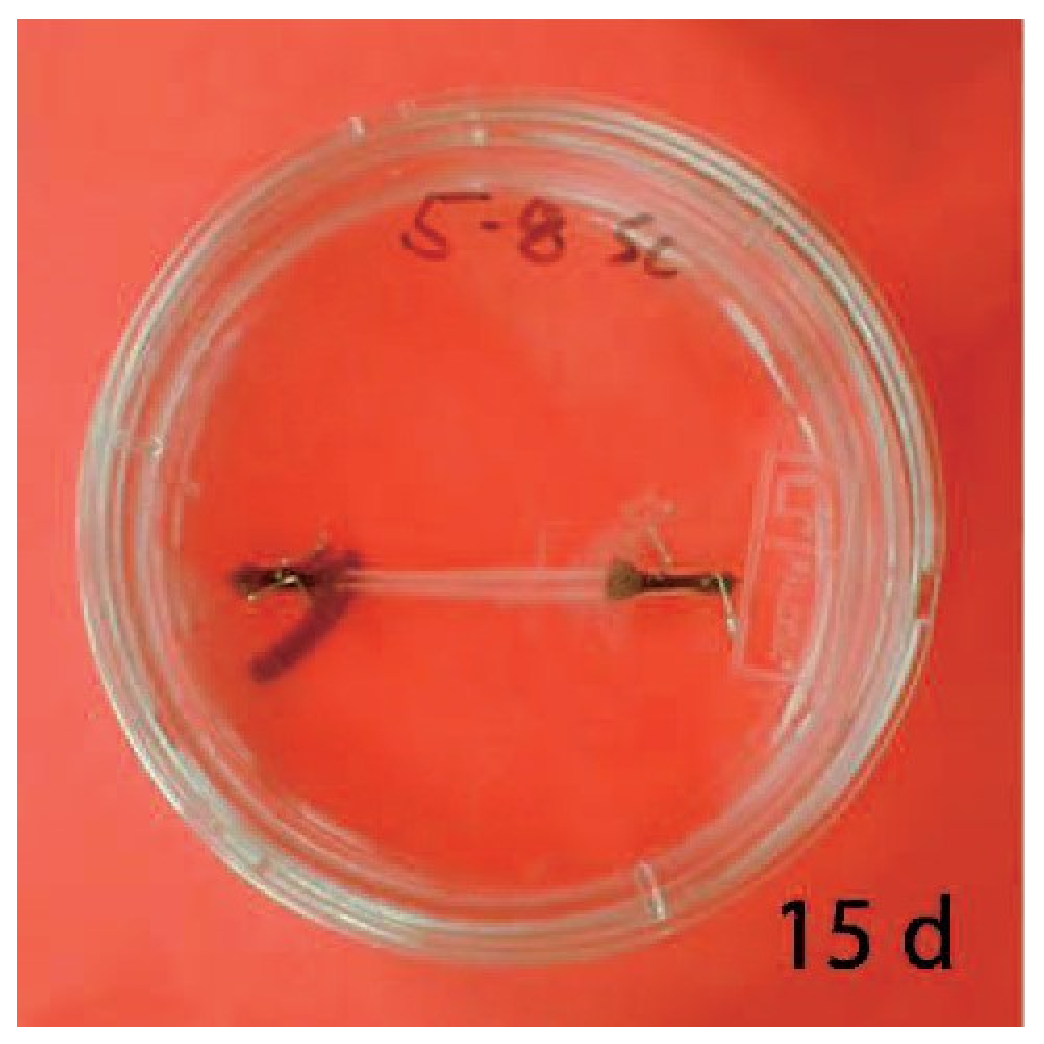
\includegraphics[width=10.00cm]{images/experiments/one-construct}
\caption{Engineered tendon constructs. See \citet{Calve:04} for
  details.} 
\label{engconst}
\end{figure}

\begin{figure}[ht]
  \centering
  \psfrag{D}{\small$1.1284$ mm}
  \psfrag{H}{\small$12.0$ mm}
  {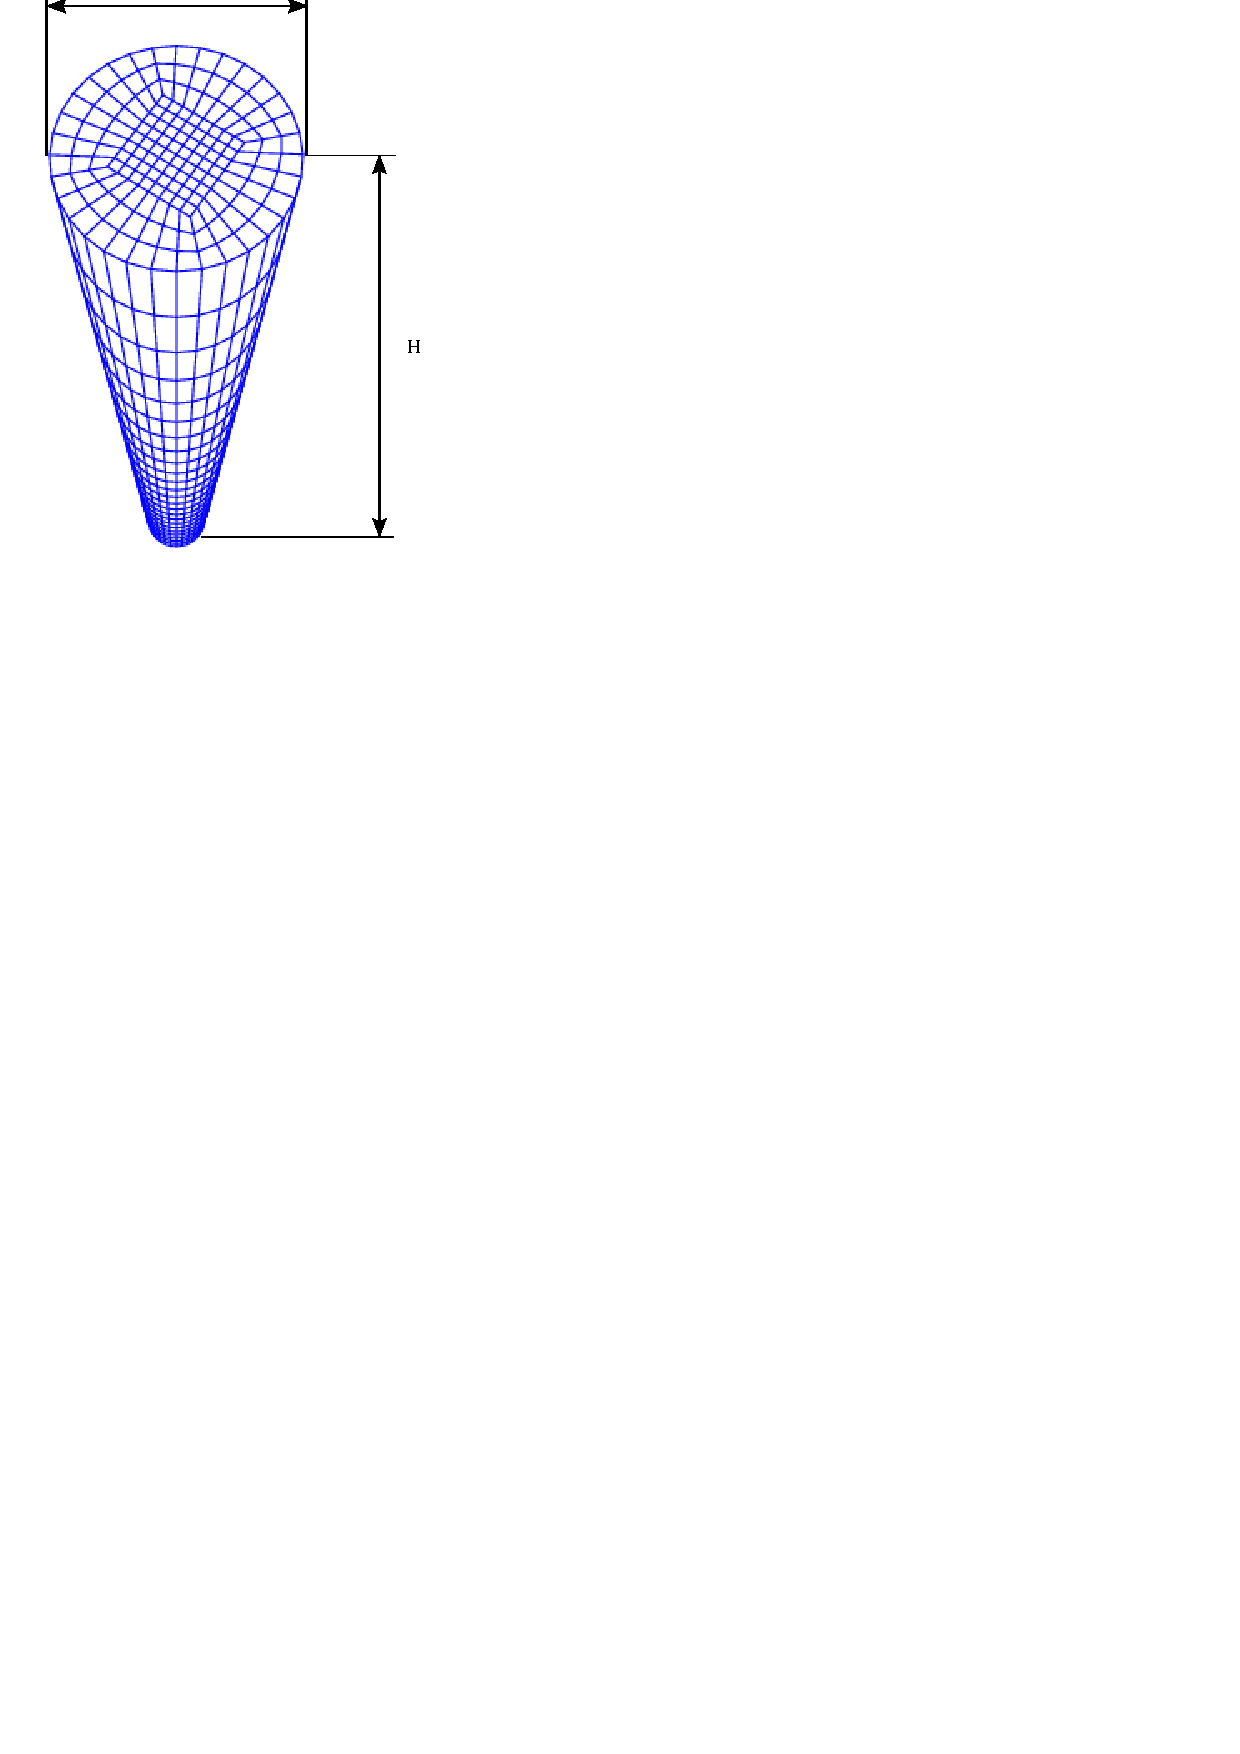
\includegraphics[width=5cm]{images/examples/lagrangian/mesh}}
  \caption{The finite element mesh used in the computations.}
  \label{egmesh}
\end{figure}

The theory presented in the preceding sections results in a system of
non-linear, coupled partial differential equations. A finite element
formulation employing a staggered scheme based upon operator splits
\cite{Armero-poroplasticity:99,Garikipatiox2:01} has been implemented
in {\tt FEAP} \citep{feapmanual} to solve the coupled problem. As an
example, in the biphasic problem involving solid and fluid
phases only, the basic solution scheme involves keeping the displacement
field fixed while solving for the concentration fields using the mass
transport equations. The resulting concentration fields are then fixed
to solve the mechanics problem. This procedure is repeated until the
resulting fields satisfy the differential equations within a specified
numerical tolerance.

The following examples aim to demonstrate the mathematical formulation
and aspects of the coupled phenomena as the tissue grows. The model
geometry, based on our engineered tendon constructs (see
Figure~\ref{engconst} and \citet{Calve:04}), is a cylinder 12 mm in length and 1 mm$^2$ in
cross-sectional area. The corresponding finite element mesh using
hexahedral elements, is shown in Figure~\ref{egmesh}.

The following numerical examples involve solution of a common set of
partial differential equations. The constutive models, however, vary as we
demonstrate the behaviour engendered by the many modelling
assumptions discussed in the paper. The balance of linear momentum
that we solve is (\ref{linearmombalance}) summed for $\iota =
\mathrm{c,f}$, with the constraint in (\ref{qrelation}) imposed. The
absence of significant acceleration in the problems under 
consideration allows us to solve the balance of linear momentum   
quasi-statically. The fluid mass balance equation is solved in the current
configuration, i.e. (\ref{massbalcurr}) for $\iota = \mathrm{f}$, but 
mass balance for the solid collagenous phase is solved in the
reference configuration, i.e. (\ref{massbalance1}) for $\iota =
\mathrm{c}$.  Mass balance for the solute is also solved in the
current configuration, but using the stabilized scheme in weak
form (\ref{stabilizedmassbal}). The Backward 
Euler algorithm is used for all mass transport equations. The
constitutive relation for the solid collagen follows
(\ref{wlcmeq}). The constitutive relation for the fluid stress follows
(\ref{Pf}) with 
\begin{equation}
h(\rho^\mathrm{f}) =
\frac{1}{2}\kappa^\mathrm{f}\left(\frac{\rho_{0_\mathrm{ini}}^\mathrm{f}}{\rho^\mathrm{f}}
- 1\right)^2,
\end{equation}

\noindent where $\kappa^\mathrm{f}$ is the fluid bulk modulus. The
tissue is modelled as being fluid saturated in $\Omega_t$ at $t = 0$,
i.e. (\ref{saturation}$_1$) holds with
$\rho^\mathrm{f}_{0_\mathrm{sat}} =
\rho^\mathrm{f}_{0_\mathrm{ini}}$. However, the tissue is allowed to 
become unsaturated in $\Omega_t$ for $t > 0$ due to void formation. Then,
the conditions set out in (\ref{cavitation})
apply. The chemical potential is then given by
(\ref{fickeanmobility}). The numerical examples that follow discuss further
specialization of the constitutive relations to other cases discussed
in the preceding sections. The numerical values of parameters\footnote{The
  mobility tensor reported in Table~\ref{parameters} is an
  order-of-magnitude estimate 
  recalculated from \citet{Hanetal:2000} to correspond to the 
  mobility used in this paper. These authors reported a mean value of
  $0.927\times 10^{-14}$ s, with a range of $1.14\times
  10^{-14}--0.58\times 10^{-14}$ s in terms of the mobility used
  here. Theirs is the mobility parallel to the fiber direction in
  Rabbit Achilles tendon. Our usage of it is as an isotropic
  mobility. Using anisotropic mobilities, or different values from the
  reported range changes the result
  quantitatively, but not qualitatively.}  that
have been used appear in Table \ref{parameters}.


Non-linear projection methods \citep{simotaylorpister:85} are used to treat the
near-incompressibility imposed by the fluid. Mixed methods, as described
in \cite{Garikipatiox2:01}, are used for stress (and strain) gradient
driven fluxes.

The initial and boundary
conditions have been chosen in order to model a few common mechanical and
chemical interventions on engineered tissue. However, we will not
attempt detailed descriptions of experiments, choosing to focus
instead on results that can be directly related to the models. A more
detailed comparison with experiments is forthcoming in a separate
communication.

\section{Examples exploring the biphasic nature of porous soft tissue}
\label{biphasic-examples-1}

In these calculations, only two phases---fluid and collagen---are
included for the mass transport and mechanics. The parameters used in the analysis
are presented in Table~\ref{parameters}. 

%The mixing entropy of fluid in the mixture with collagen is
%written as $\eta_{\mathrm{mix}}^{f} = -\frac{k}{\sM^\mathrm{f}}
%\mathrm{log} (\frac{\rho^\mathrm{f}} {\rho})$, where
%$\sM^\mathrm{f}$ is the molecular weight of the fluid.

\subsection{Using the appropriate configuration}
\label{biphasic-examples-1}

%\subsubsection{Unbounded pinching problem}
%\label{unbounded-pinching}

\subsection{Fluxes from different driving forces}
\label{flux-driving-forces}

The following contour plots represent the stress, and various
contributions to the total flux in the early stages of loading of
the model problem. Symmetry has been employed to model a single
quadrant of the cylinder.

The longitudinal stress, $\sigma_{33}$ in Figure \ref{stressfig}
arises from the stretch and the evolution in concentration.
\begin{figure}[ht]
\begin{minipage}[t]{7.5cm}
{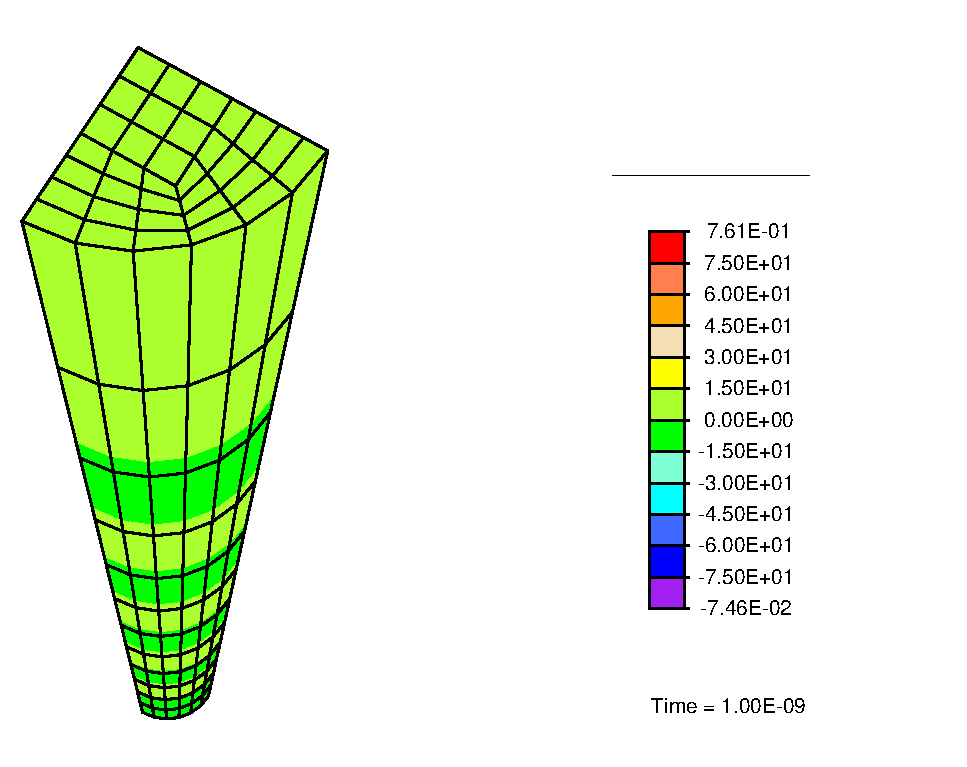
\includegraphics[width=7.5cm]{images/examples/lagrangian/preliminary/S33-1}} \hskip 3cm (a) 
\end{minipage}
\begin{minipage}[t]{7.5cm}
{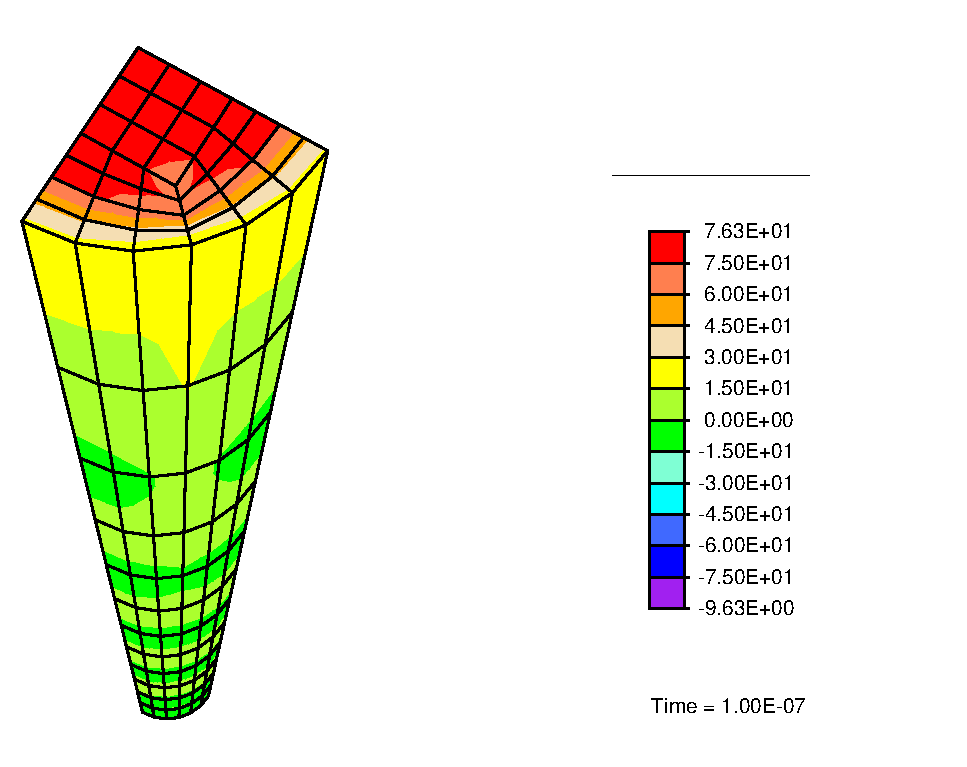
\includegraphics[width=7.5cm]{images/examples/lagrangian/preliminary/S33-100}} \hskip 3cm (b)
\end{minipage}
\caption{Longitudinal Cauchy stress, $\sigma_{33}$ (Pa) at $1
\,\mathrm{nanosec.}$ and $100\,\mathrm{nanosec.}$ after the
beginning of loading.} \label{stressfig}
\end{figure}

\begin{figure}[ht]
\begin{minipage}[t]{7.5cm}
{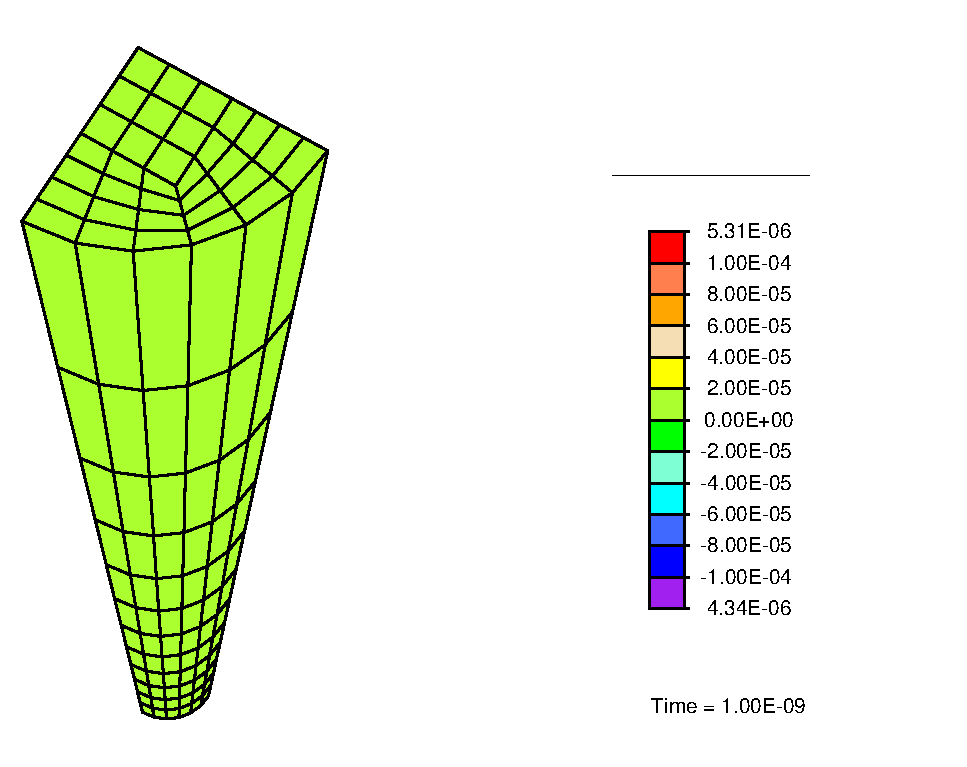
\includegraphics[width=7.5cm]{images/examples/lagrangian/preliminary/M1-1}} \hskip 3cm (a)
\end{minipage}
\begin{minipage}[t]{7.5cm}
{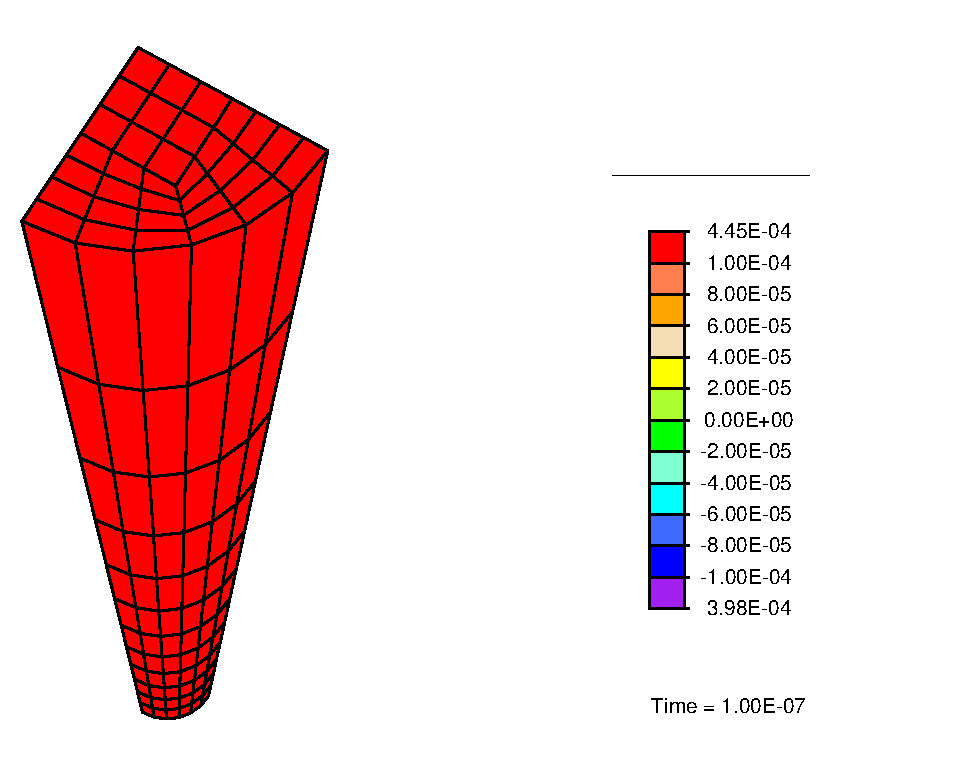
\includegraphics[width=7.5cm]{images/examples/lagrangian/preliminary/M1-100}} \hskip 3cm (b)
\end{minipage}
\caption[Stress gradient-driven flux]{Stress gradient-driven flux
($\mathrm{kg.m}^{-2}\mathrm{sec}$) in the $\be_3$ direction at $1
\,\mathrm{nanosec.}$ and $100\,\mathrm{nanosec.}$ after the
beginning of loading. The positive values indicate an upward flux
corresponding to a tensile $\sigma_{33}$ wave travelling
downwards.} \label{M1fig}
\end{figure}

\begin{figure}[ht]
\begin{minipage}[t]{7.5cm}
{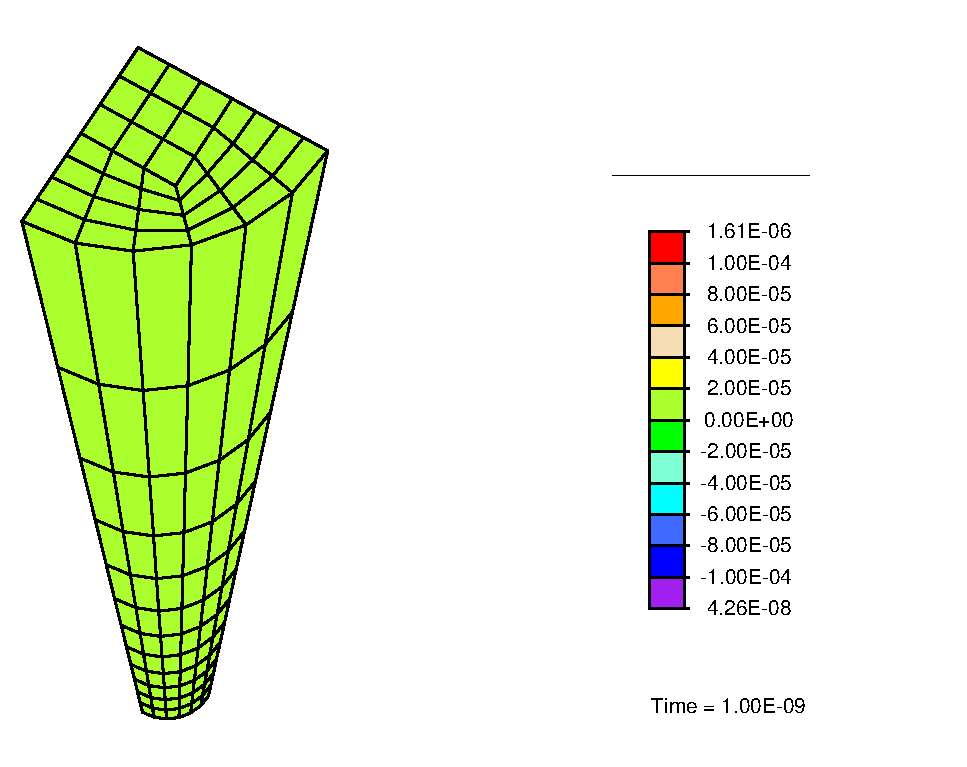
\includegraphics[width=7.5cm]{images/examples/lagrangian/preliminary/M2-1}} \hskip 3cm (a)
\end{minipage}
\begin{minipage}[t]{7.5cm}
{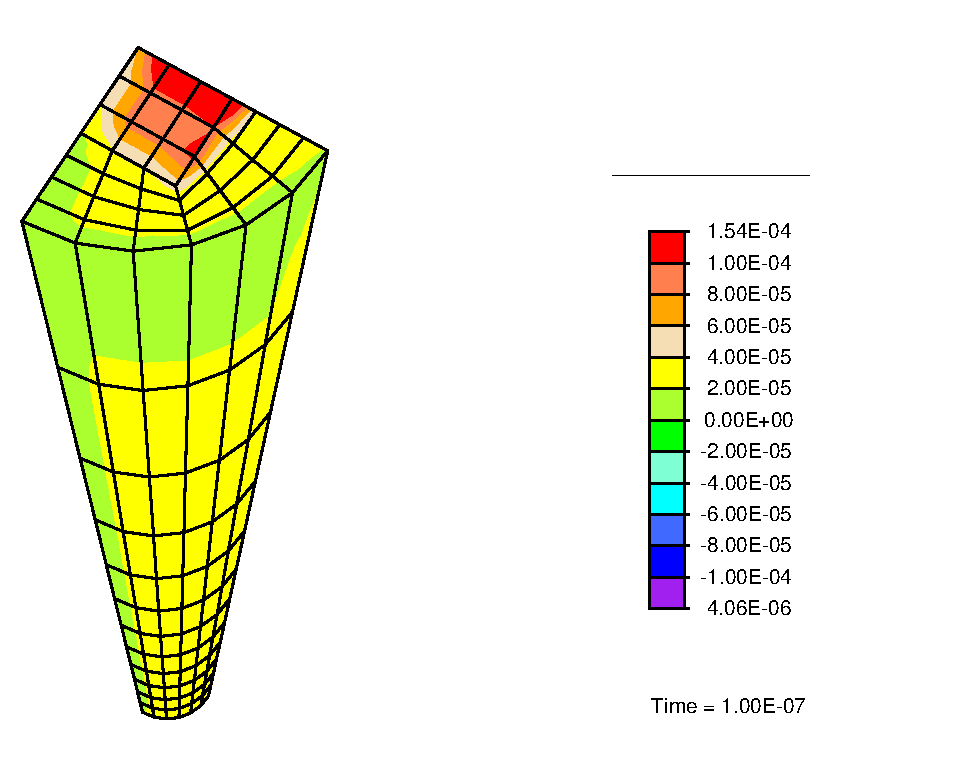
\includegraphics[width=7.5cm]{images/examples/lagrangian/preliminary/M2-100}} \hskip 3cm (b)
\end{minipage}
\caption{Internal energy gradient-driven flux,
($\mathrm{kg.m}^{-2}\mathrm{sec}$) in the $\be_3$ direction at $1
\,\mathrm{nanosec.}$ and $100\,\mathrm{nanosec.}$ after the
beginning of loading. The positive values indicate an upward flux.
This corresponds to a lower energy near the top of the cylinder as
the tensile stress ($\sigma_{33}$) wave travels downward and
relaxes some of the strain energy of contraction.} \label{M2fig}
\end{figure}

\begin{figure}[ht]
\begin{minipage}[t]{7.5cm}
{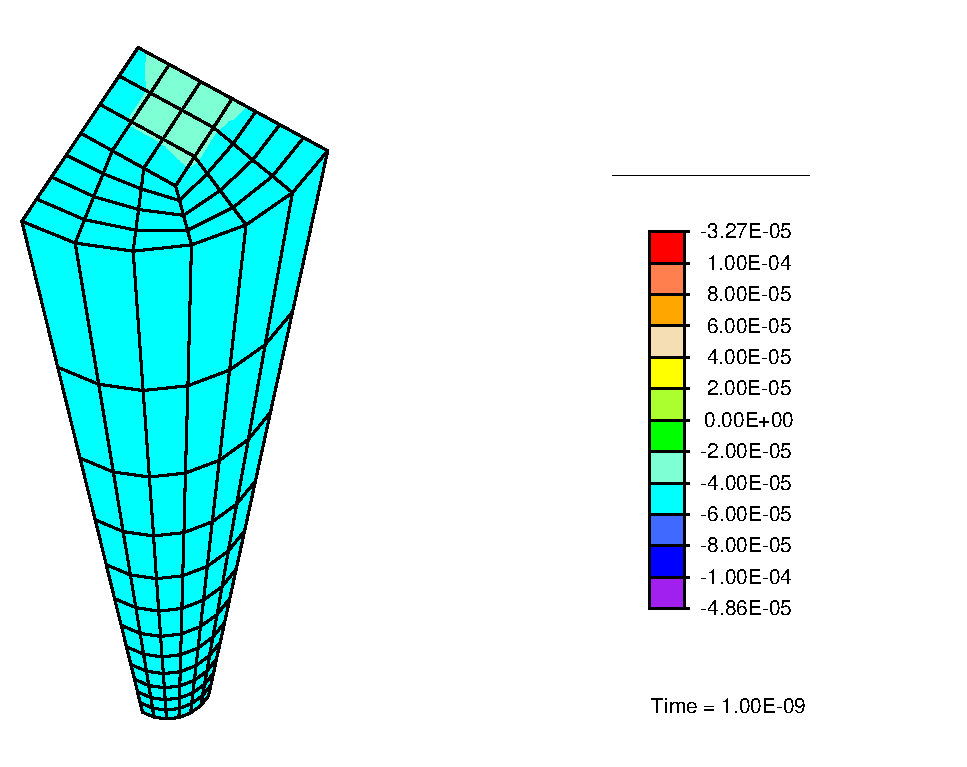
\includegraphics[width=7.5cm]{images/examples/lagrangian/preliminary/M3-1}} \hskip 3cm (a)
\end{minipage}
\begin{minipage}[t]{7.5cm}
{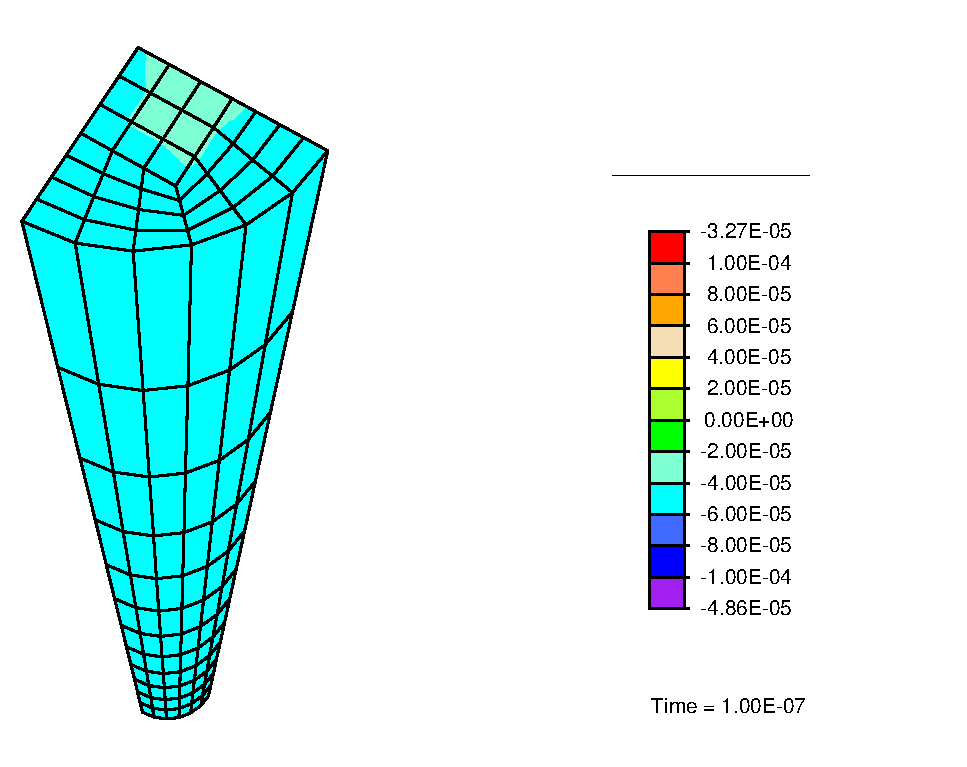
\includegraphics[width=7.5cm]{images/examples/lagrangian/preliminary/M3-100}} \hskip 3cm (b)
\end{minipage}
\caption{Gravity-driven flux ($\mathrm{kg.m}^{-2}\mathrm{sec}$) in
the $\be_3$ direction at $1 \,\mathrm{nanosec.}$ and
$100\,\mathrm{nanosec.}$ after the beginning of loading. The
negative values indicate a downward flux, due to the action of
gravity.} \label{M3fig}
\end{figure}

\begin{figure}[ht]
\begin{minipage}[t]{7.5cm}
{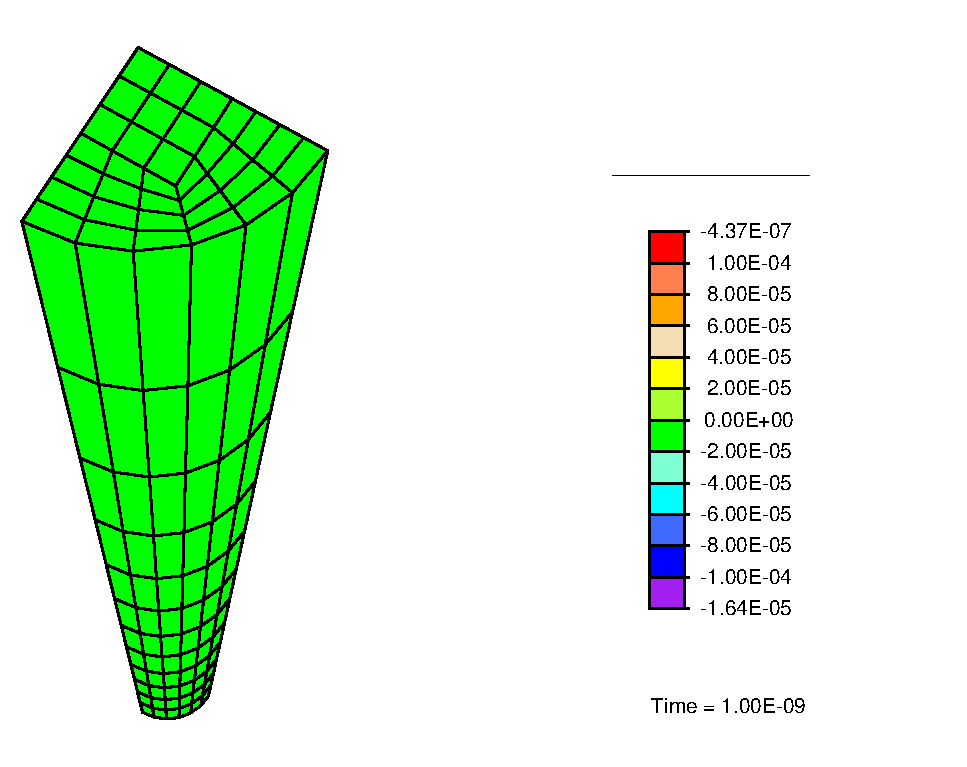
\includegraphics[width=7.5cm]{images/examples/lagrangian/preliminary/M4-1}} \hskip 3cm (a)
\end{minipage}
\begin{minipage}[t]{7.5cm}
{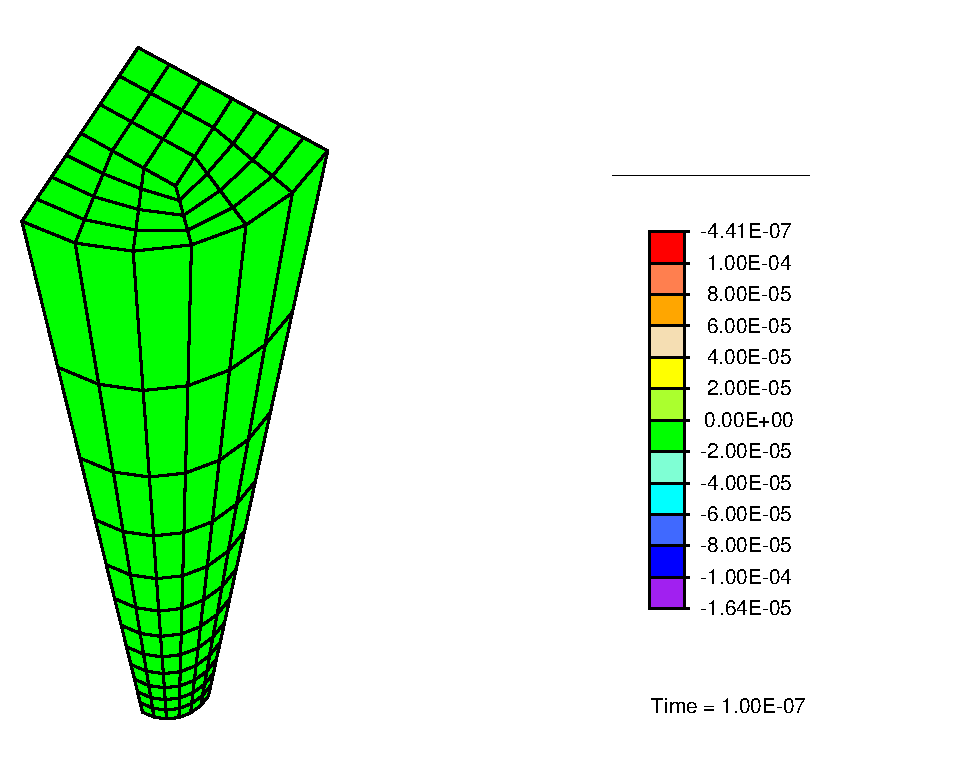
\includegraphics[width=7.5cm]{images/examples/lagrangian/preliminary/M4-100}} \hskip 3cm (b)
\end{minipage}
\caption{Inertia-driven flux ($\mathrm{kg.m}^{-2}\mathrm{sec}$) in
the $\be_3$ direction at $1 \,\mathrm{nanosec.}$ and
$100\,\mathrm{nanosec.}$ after the beginning of loading. The
negative values indicate a downward flux as the tissue accelerates
upward.} \label{M4fig}
\end{figure}

\begin{figure}[ht]
\begin{minipage}[t]{7.5cm}
{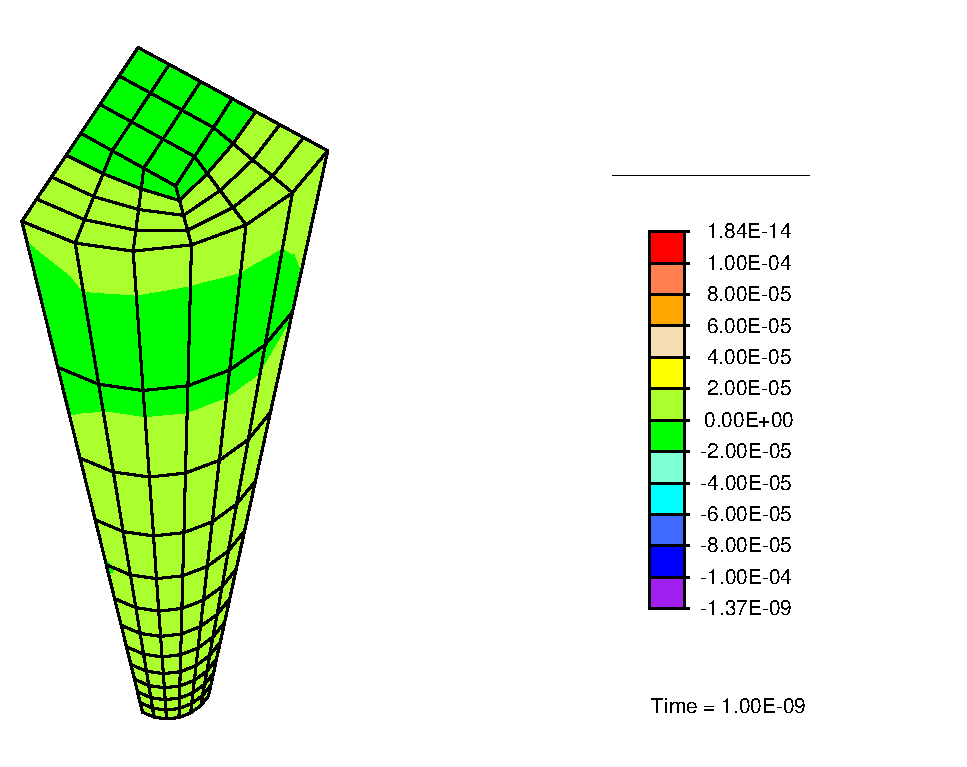
\includegraphics[width=7.5cm]{images/examples/lagrangian/preliminary/M5-1}} \hskip 3cm (a)
\end{minipage}
\begin{minipage}[t]{7.5cm}
{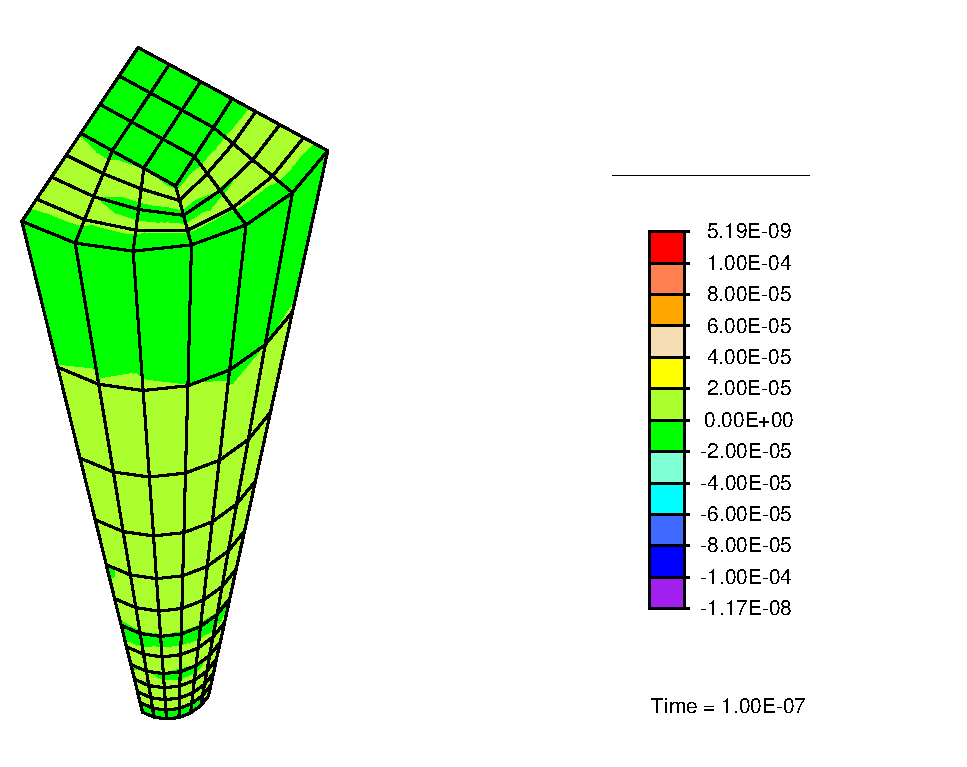
\includegraphics[width=7.5cm]{images/examples/lagrangian/preliminary/M5-100}} \hskip 3cm (b)
\end{minipage}
\caption{Concentration gradient-driven flux
($\mathrm{kg.m}^{-2}\mathrm{sec}$) in the $\be_3$ direction at $1
\,\mathrm{nanosec.}$ and $100\,\mathrm{nanosec.}$ after the
beginning of loading. Note that the maximum and minimum values are
many orders of magnitude lower than for the other flux
contributions reported above. This is a demonstration of mechanics
influences dominating diffusion over the classical concentration
gradient contribution.} \label{M5fig}
\end{figure}

\begin{figure}[ht]
\begin{minipage}[t]{7.5cm}
{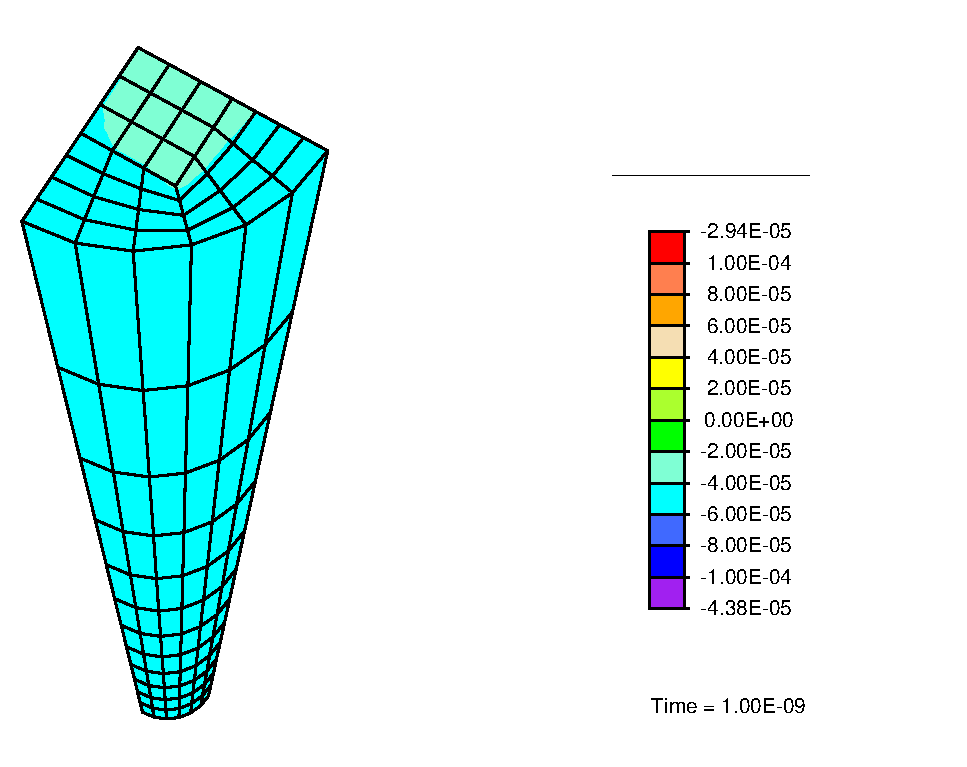
\includegraphics[width=7.5cm]{images/examples/lagrangian/preliminary/M-1}} \hskip 3cm (a)
\end{minipage}
\begin{minipage}[t]{7.5cm}
{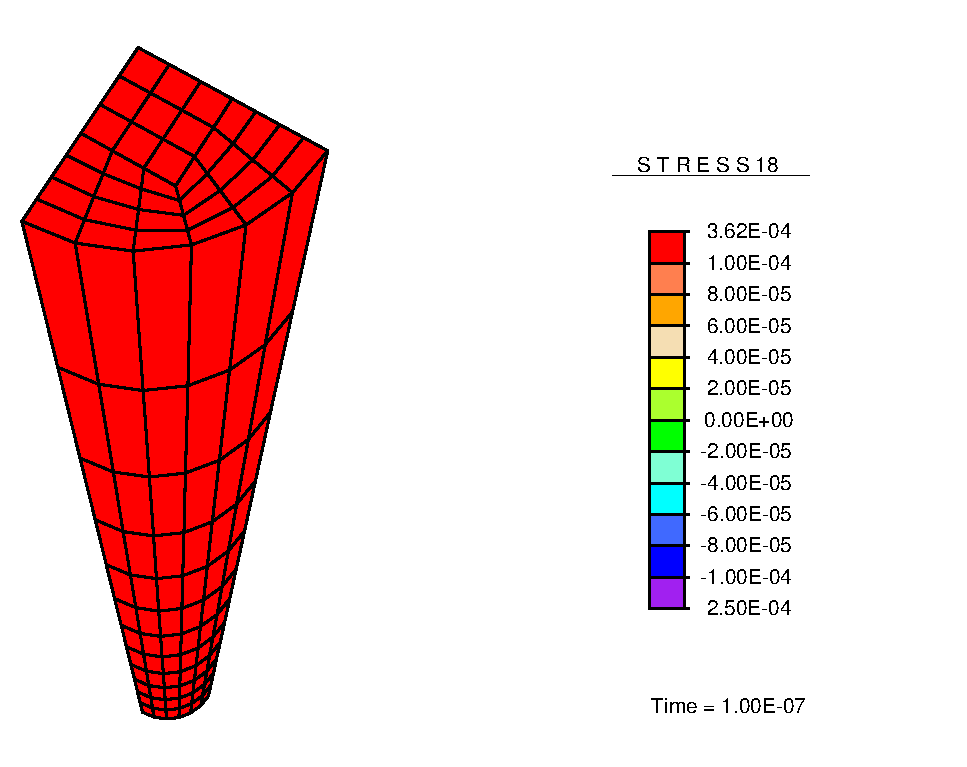
\includegraphics[width=7.5cm]{images/examples/lagrangian/preliminary/M-100}} \hskip 3cm (b)
\end{minipage}
\caption{Total flux ($\mathrm{kg.m}^{-2}\mathrm{sec}$) in the
$\be_3$ direction at $1 \,\mathrm{nanosec.}$ and
$100\,\mathrm{nanosec.}$ after the beginning of loading. The
positive values indicate an upward flux, dominated by the stress
gradient driven contribution.} \label{Mfig}
\end{figure}

The flux contributions in Figures \ref{M1fig}--\ref{Mfig} can be
summarized as follows: The fluid flux is dominated by the
contribution from the stress gradient in the $\be_3$ direction.
The latter arises as the stress ($\sigma_{33}$) wave of tension
travels down the cylinder in the first few microseconds after
application of the load (the time taken to travel the length of
the cylinder is $12 \,\mu\mathrm{sec}$). Additionally, as the
fluid concentration changes due to the flux, it causes a further
change in the stress (Section \ref{sect5}). Other flux terms are
qualitatively sensible; i.e., their directions are consistent with
the physics of the problem, as argued in each of the figure
captions\footnote{In order to compare the flux contributions, they
have all been plotted on the same scale: $-1\times
10^{-4}--1\times 10^{-4} \,\mathrm{kg.m}^{-2}\mathrm{sec}$.
However the plots also show the maximum and minimum field values
at the top and bottom of the legend bars. These values represent a
better comparison of the relative flux magnitudes.}. There is some
loss of axial symmetry in a few of the plots due to the coarseness
of the finite element mesh for this example. It appears that
spatial oscillations in the solution lead to a further loss of
symmetry in Figures \ref{M2fig}b--\ref{M3fig}b and \ref{Mfig}a.
These oscillations arise due to large and dominant advective
terms, and need to be remedied by stabilized finite element
methods. Here, we only aim to demonstrate that various driving
forces for mass transport are in agreement with their theoretical
underpinnings in the paper. The resorption of the solid phase is
shown indirectly in Figure \ref{Pifig}. A positive fluid source,
$\Pi^\mathrm{f}$, means that $\Pi^\mathrm{s} < 0$. Since
$\Pi^\mathrm{s}$ is the only term balancing
$\partial\rho_0^\mathrm{s}/\partial t$ [see (\ref{massballocA})],
it follows that $\partial\rho_0^\mathrm{s}/\partial t < 0$.

\begin{figure}[ht]
\begin{minipage}[t]{7.5cm}
{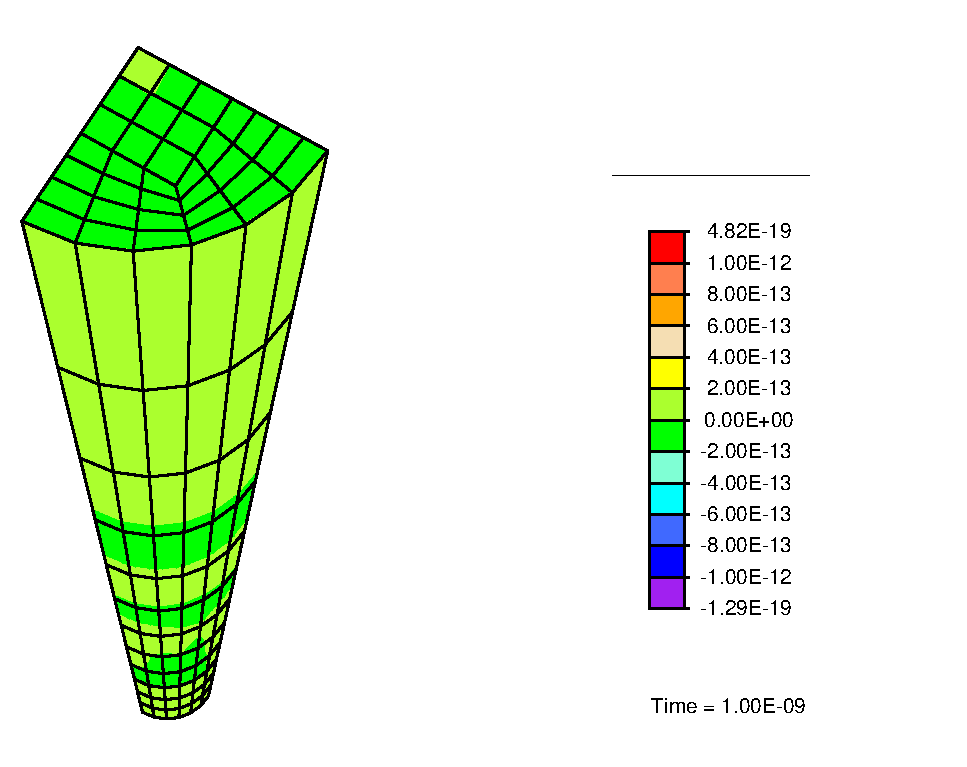
\includegraphics[width=7.5cm]{images/examples/lagrangian/preliminary/Pi-1}} \hskip 3cm (a)
\end{minipage}
\begin{minipage}[t]{7.5cm}
{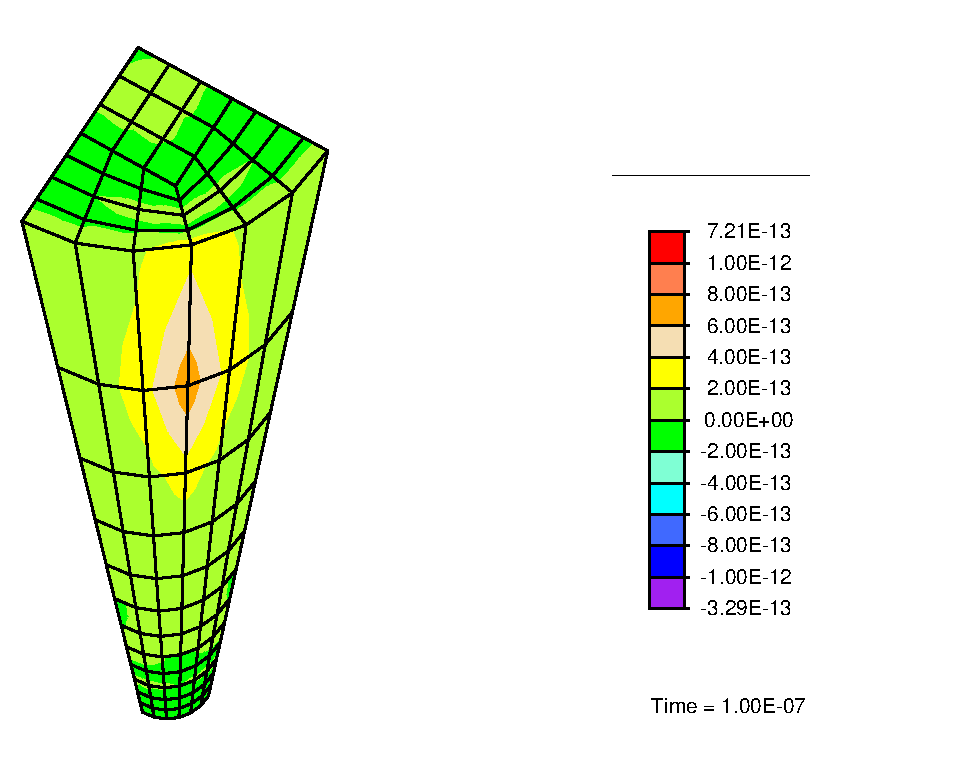
\includegraphics[width=7.5cm]{images/examples/lagrangian/preliminary/Pi-100}} \hskip 3cm (b)
\end{minipage}
\caption{Rate of fluid production, $\Pi^\mathrm{f}$
($\mathrm{kg.m}^{-3}.\mathrm{sec}^{-1}$), at $1
\,\mathrm{nanosec.}$ and $100\,\mathrm{nanosec.}$ after the
beginning of loading. The positive values indicate that the local
fluid concentrations have fallen below their initial values.}
\label{Pifig}
\end{figure}

\subsection{The tendon under constriction}
\label{constriction-1}

In this example, the tendon immersed in a bath is subjected to the same
constrictive radial load as in Section~\ref{enzyme_kinetics_eg}. Since
that example demonstrated an insignificant amount of local collagen production
over this time scale, we have simplified the
problem by setting the source term $\Pi^\mathrm{c} = 0$. The total
duration of the simulation is 
10~s, and the radial strain is applied as a displacement boundary
condition, increasing linearly from no strain initially to the maximum
strain at time $t = 1~\mathrm{s}$. Again,
both the initial collagen 
concentration and the initial fluid concentration are 500~kg.m$^{-3}$
at every point in the tendon. This tendon is exposed to a bath where
the fluid concentration is 500~kg.m$^{-3}$.

While solving the balance of momentum for the biphasic problem
of the solid collagen and a fluid phase, we currently treat the
tissue as a single entity and employ a summation of
Equation~(\ref{linearmombalance}) over both species. Additionally,
condition~(\ref{qrelation}) allows us to avoid constitutive
prescription of the momentum transfer terms between solid collagen and
fluid phases,
$\bq^\mathrm{c}$ and $\bq^\mathrm{f}$. This facilitates considerable
simplification of the 
problem, but such a treatment requires additional assumptions on the
detailed deformation of the constitutive phases of the tissue. An
explicit assumption we have drawn on thus far is the equality of
the deformation gradient of the solid collagen and pore spaces,
allowing us to use the deformation gradient
$\bF$, suitably decomposed to account for change in fluid
concentration, to model the fluid stress. This assumption and its 
consequences have been discussed in Sections \ref{bomass},
\ref{growthkinem}, \ref{satswel}, \ref{compfluid}, \ref{tensionfluid}
and \ref{incompfluid}. Since the imposition of a common deformation gradient
results in an upper bound for the 
effective stiffness of the tissue and magnitudes of the fluxes
established, we refer to it as the {\em upper bound model}. This
assumption plays a fundamental role in determining the fluid flux driven
by the fluid stress gradient.

\begin{figure}[ht]
  \centering
      {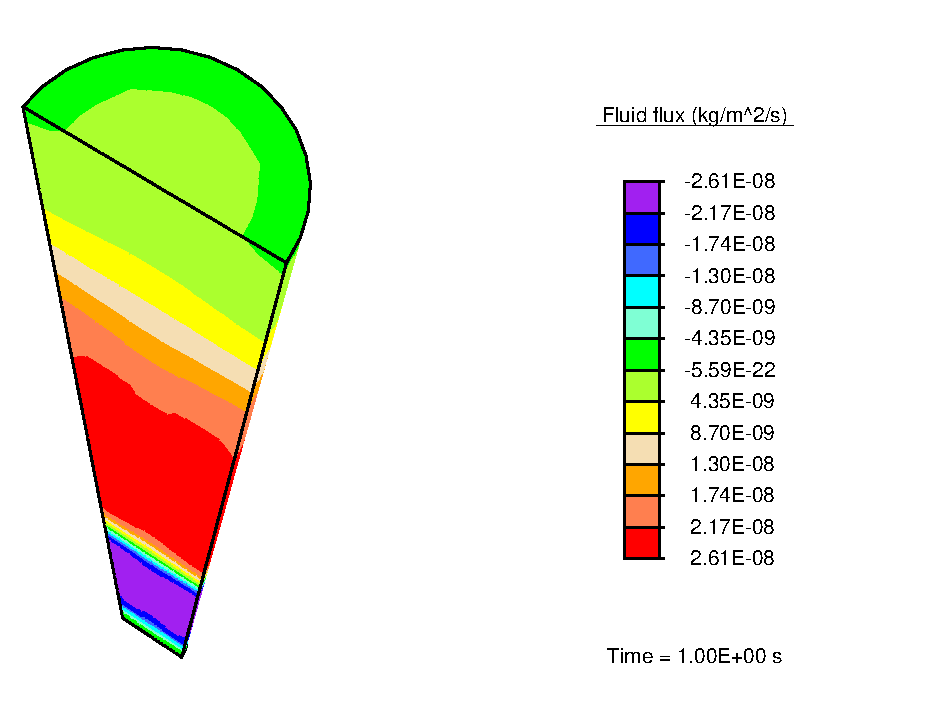
\includegraphics[width=10.00cm]{images/examples/lagrangian/constriction/upper-bound-flux}}
      \caption{{\em Upper bound} fluid flux (kg.m$^{-2}$.s$^{-1}$) in
        the vertical direction at time $t=1$~s.}
      \label{eg2flux}
\end{figure}

\noindent For this upper bound model, Figure~\ref{eg2flux} shows the fluid flux in
the vertical direction at the final stage of the constriction phase of
the simulation, i.e. at time $t=1$~s. The flux values are positive
above the central plane, forcing fluid upward, and negative below,
forcing fluid fluid downward. This stress-gradient induced fluid flux
results in a reference concentration distribution of the fluid that is
higher near the top and bottom faces, as seen in Figure~\ref{eg2conc}.

\begin{figure}[ht]
  \centering
      {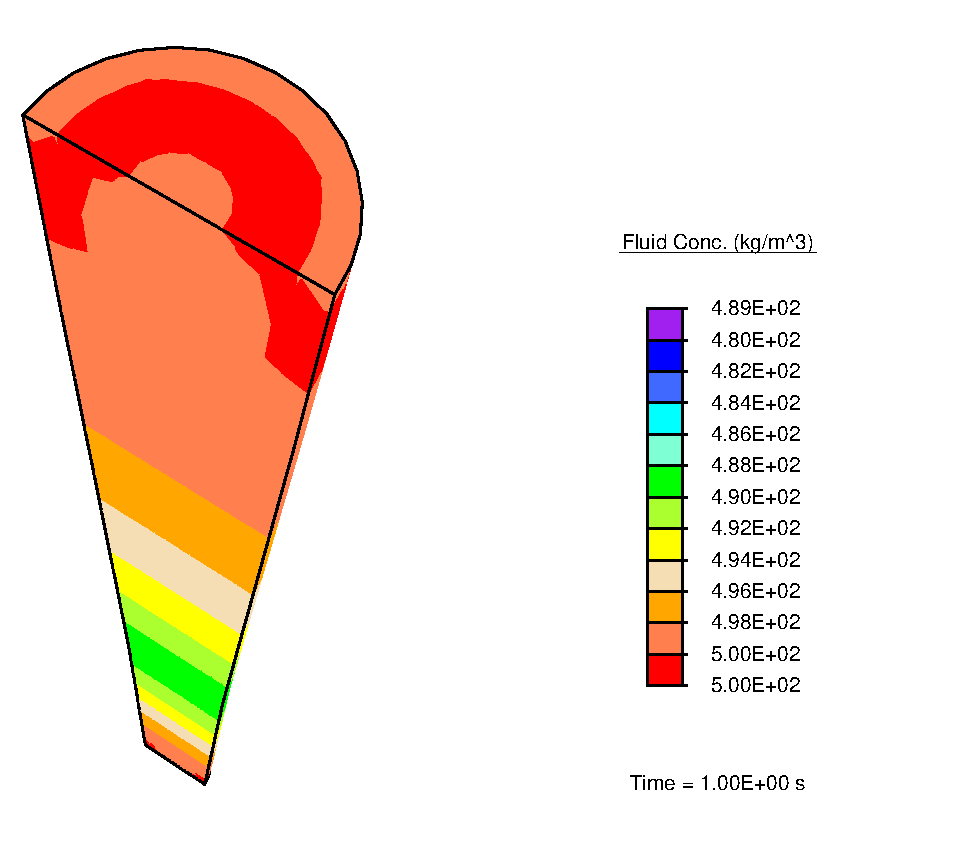
\includegraphics[width=10.00cm]{images/examples/lagrangian/constriction/fluid-concentration}}
      \caption{Reference fluid concentration (kg.m$^{-3}$) at time
      $t=1$~s.}
      \label{eg2conc}
\end{figure}

As a result, these regions would have seen a higher production of
collagen, or preferential growth, in the presence of non-zero source
terms. As discussed in Section~\ref{curr-ref-mb}, the mass transport
equations are solved in the current configuration, where physical
boundary conditions can be set directly. The values reported in
Figure~\ref{eg2conc} are pulled back from the current
configuration. The current concentrations do not change for this
boundary value problem. 

Solving a problem of this nature in the
reference configuration using $\rho_0^\mathrm{f} = $ const. as the
boundary condition to represent immersion of the tendon in a fluid bath
yields non-physical results, such as an unbounded flow. This occurs
since the imposed strain gradient causes a stress gradient in the
fluid that does not decay. The imposed boundary condition on $\rho_0^\mathrm{f}$
prevents a redistribution of concentration that would have provided an
opposing, internal gradient of stress, which in turn would drive the
flux to vanish.

The tendon is held fixed in the radial direction after the
constriction phase. The applied stress sets up a pressure wave in the
fluid travelling toward the top and bottom faces. As the fluid leaves
these surfaces, we observe that the tendon relaxes. This is seen in
Figure~\ref{topdisp}, which plots the vertical displacement of the top
face with time, showing a decrease in height of the tendon after the
constriction phase. We keep the centre of the bottom face of the
tendon fixed.

\begin{figure}[ht]
  \centering
      {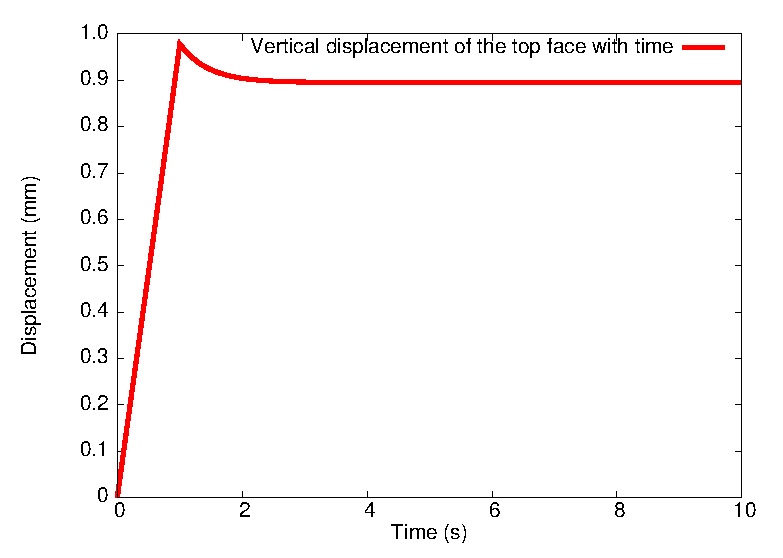
\includegraphics[width=10.00cm]{images/examples/lagrangian/constriction/top-vertical-displacement}}
      \caption{Relaxation of the top face of the tendon after the
      constriction phase.}
      \label{topdisp}
\end{figure}

In order to define a range of the magnitude of fluid flux, we now
introduce the {\em lower bound model} (on effective stiffness of the
tissue and, consequently, the magnitude of the fluid flux). For this lower bound, we
replace the earlier strain homogenisation requirement with a stress
homogenisation requirement, {\em viz.} equating the hydrostatic stress
of the solid phase and the fluid pressure in the current
configuration:

\begin{equation}
p^{\mathrm{f}}=\frac{1}{3} \mathrm{\small{tr}}[\Bsigma^{c}],
\label{equalpr}
\end{equation}

\noindent where $p^{\mathrm{f}}$ is the fluid pressure in the current
configuration, $\mbox{\small{tr}[\textbullet]}$ is the trace operator, and
$\Bsigma^{c}=\frac{1}{\mathrm{J^{c}}} \bP^{\mathrm{c}}
\bF^{\mathrm{c}^{\mathrm{T}}}$ is the Cauchy stress of the solid. The
Cauchy stress of an ideal fluid can be defined from its current
pressure as \mbox{$\Bsigma^{f}= p^{\mathrm{f}} \bone$.}
Figure~{\ref{lowerbound}} reports the value of the vertical flux under
the lower bound modelling assumption, using boundary conditions identical to the
previous calculation at time $t=1$~s, the final stage of the
constriction phase of the simulation. 


\begin{figure}[ht]
  \centering
      {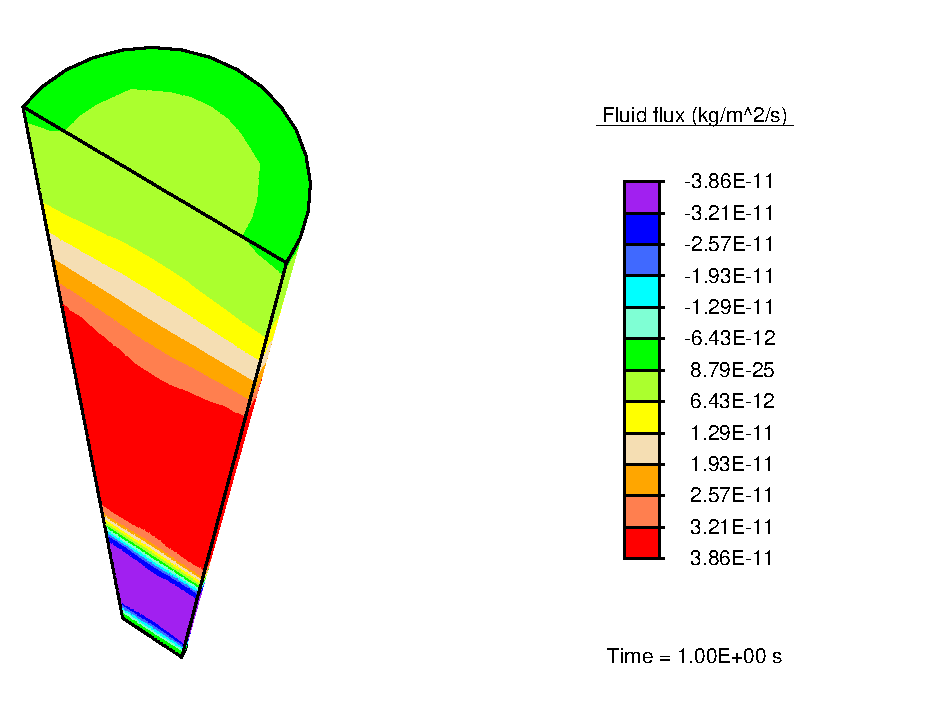
\includegraphics[width=10.00cm]{images/examples/lagrangian/constriction/lower-bound-flux}}
      \caption{{\em Lower bound} fluid flux (kg.m$^{-2}$.s$^{-1}$) in
        the vertical direction at time $t=1$~s.}
      \label{lowerbound}
\end{figure}

The fluid flux values reported in Figures~\ref{eg2flux} and
\ref{lowerbound} (corresponding to the upper and lower bound modelling
assumptions, respectively) are qualitatively similar, but differ by
about three orders of magnitude. This wide range points to the
importance of imposing the appropriate mechanical coupling model
between interacting phases. Note, however, that we have computed
bounds for the 
range of possible fluid flux values under the specified mechanical
loading. Recall, furthermore, that the example in Section
\ref{enzyme_kinetics_eg} used the upper bound model, and yet resulted
in no discernible advective solute transport. This suggests strongly
that, given the parameters in Table \ref{parameters}, convective
transport of nutrients in tendons is dominated by diffusive
transport. In future work, we will detail models that result in precise
field values for the fluxes, which will replace the upper and lower
bounds discussed here.  


This numerical example also points to the fact that a convenient
measure of the strength of 
coupling between the mechanics and mass transport equations is the
ratio of the variation in hydrostatic stress of the fluid to that of
the solid. In the lower bound case, where the fluid response is
defined by Equation~(\ref{equalpr}), it is instructive to note that
this ratio is unity. As a result, it is seen that the lower bound case
exhibits significantly weaker coupling than the upper bound case. In
the latter, variation in the common deformation gradient, $\delta
\bF$, causes instantaneous variation in \mbox{$\delta p^{\mathrm{f}} \approx
  O(\kappa^{\mathrm{f}} \delta \bF:\bF^{-\mathrm{T}})$} and in
\mbox{$\frac{1}{3} \delta\mathrm{\small{tr}}[\Bsigma^{c}] \approx
  O(\kappa^{\mathrm{c}} \delta \bF:\bF^{-\mathrm{T}})$}, where
$\kappa^{\mathrm{c}}$ is the bulk modulus of the solid. The ratio
$\frac{\delta p^{\mathrm{f}}}{\frac{1}{3} \delta
  \mathrm{\small{tr}}[\Bsigma^{c}]}$ is therefore \mbox{$\approx
O(\kappa^{\mathrm{f}}/\kappa^{\mathrm{c}}) \gg 1$}.

The strength of coupling between the equations plays a principal role
in the rate of convergence of the solution, as observed in
Table~\ref{resnorms}, where the residual norms of the equilibrium
equation (and
corresponding CPU times in seconds for an Intel\textregistered Xeon
3.4 GHz machine) are reported for the first 8 iterations of each of
the two cases. Recall that the staggered scheme involves solution of
the mechanics equation 
keeping the concentrations fixed, and the mass transport equation
keeping the displacements fixed, in turn, until the solution
converges. The table does not report the value of the residual norms
arising from the solution of the mass transport equation for the
fluid, which occurs after each reported solve of the of the mechanics
equation. Although the initial mechanics residual norms in successive
passes are decreasing linearly in both cases, the rapid decrease in
this quantity in
the weakly-coupled case ensures convergence in far fewer iterations
than the strongly coupled case. Thus, the corresponding CPU times
reported are also lower for the weakly coupled case. This is
advantageous. In addition to being more physical, as argued at
the beginning of Section \ref{swelling} immediately below, the lower
bound, weakly-coupled case makes it feasible to drive 
problems to longer, physiologically-relevant time-scales through the use
of larger time steps.

\begin{table}
\centering
\begin{tabular}{|r|c|c|c|c|}
  \hline
  Pass & \multicolumn{2}{c|}{Strongly coupled} &
         \multicolumn{2}{c|}{Weakly coupled}\\
  \cline{2-5} & Residual & CPU (s) & Residual & CPU (s)\\
  \hline\hline 
1     & $ 2.138\times 10^{-02}$ &   29.16   & $6.761 \times 10^{-04}$  &    28.5 \\
      & $ 3.093\times 10^{-04}$ &   55.85   & $1.075 \times 10^{-04}$  &    55.1 \\
      & $ 2.443\times 10^{-06}$ &   82.37   & $4.984 \times 10^{-06}$  &    81.8 \\
      & $ 2.456\times 10^{-08}$ &  109.61   & $1.698 \times 10^{-08}$  &   107.9 \\
      & $ 4.697\times 10^{-14}$ &  135.83   & $3.401 \times 10^{-13}$  &   134.1 \\
      & $ 1.750\times 10^{-16}$ &  163.18   & $1.1523\times 10^{-17}$  &   161.1 \\
\hline                                    
2     & $ 5.308\times 10^{-06}$ &  166.79   & $5.971 \times 10^{-08}$  &  192.5  \\
      & $ 4.038\times 10^{-10}$ &  193.36   & $4.285 \times 10^{-11}$  &  218.6  \\
      & $ 1.440\times 10^{-14}$ &  220.45   & $2.673 \times 10^{-15}$  &  246.1  \\
      & $ 4.221\times 10^{-17}$ &  247.04   & $                    $   &  \\
\hline                                    
3     & $ 5.186\times 10^{-06}$ &  250.62   & $2.194 \times 10^{-09}$  &  277.3  \\
      & $ 3.852\times 10^{-10}$ &  277.44   & $2.196 \times 10^{-13}$  &  304.2   \\
      & $ 1.369\times 10^{-14}$ &  304.16   & $1.096 \times 10^{-17}$  &  331.6   \\
      & $ 4.120\times 10^{-17}$ &  331.47   & $                    $   &  \\
\hline                                    
4     & $ 5.065\times 10^{-06}$ &  335.16   & $8.160 \times 10^{-11}$  &  363.2 \\ 
      & $ 3.674\times 10^{-10}$ &  362.24   & $7.923 \times 10^{-15}$  &  390.2 \\
      & $ 1.300\times 10^{-14}$ &  388.79   & $                    $   &  \\
      & $ 4.021\times 10^{-17}$ &  416.08   & $                    $   &  \\
\hline                                    
5     & $ 4.948\times 10^{-06}$ &  419.59   & $3.078 \times 10^{-12}$  &  421.4 \\
      & $ 3.503\times 10^{-10}$ &  446.24   & $3.042 \times 10^{-16}$  &  448.6 \\
      & $ 1.236\times 10^{-14}$ &  473.20   & $                    $   &  \\
      & $ 3.924\times 10^{-17}$ &  500.85   & $                    $   &  \\
\hline                                    
6     & $ 4.832\times 10^{-06}$ &  504.65   & $1.179 \times 10^{-13}$  &  479.9 \\
      & $ 3.340\times 10^{-10}$ &  531.28   & $1.291 \times 10^{-17}$  &  507.0 \\
      & $ 1.174\times 10^{-14}$ &  558.17   & $                    $   &  \\
      & $ 3.829\times 10^{-17}$ &  585.27   & $                    $   &  \\
\hline                                    
7     & $ 4.720\times 10^{-06}$ &  589.01   & $4.592 \times 10^{-15}$  &  537.8 \\
      & $ 3.184\times 10^{-10}$ &  616.24   & $5.152 \times 10^{-18}$  &  564.6 \\
      & $ 1.116\times 10^{-14}$ &  643.29   & $                    $   &  \\
      & $ 3.737\times 10^{-17}$ &  670.83   & $                    $   &  \\
\hline                                    
8     & $ 4.609\times 10^{-06}$ &  674.46   & $1.816 \times 10^{-16}$  &  595.5  \\
      & $ 3.034\times 10^{-10}$ &  701.74   & $5.040 \times 10^{-18}$  &  622.3  \\
      & $ 1.060\times 10^{-14}$ &  727.74   & $                    $   &  \\
      & $ 3.646\times 10^{-17}$ &  755.58   & $                    $   &  \\
\hline
\end{tabular}
\caption{Mechanics equation residual norms and corresponding CPU times
  in seconds for the first 8 passes of each of the two cases for a
  typical time increment, $\Delta t=$ 0.1 s.}
\label{resnorms}
\end{table}

\subsubsection{Upper bound model}
\label{upper-bound}

\subsubsection{Lower bound model}
\label{lower-bound}

\subsection{A swelling problem}
\label{swelling-1}

\begin{figure}[ht]
  \centering
     {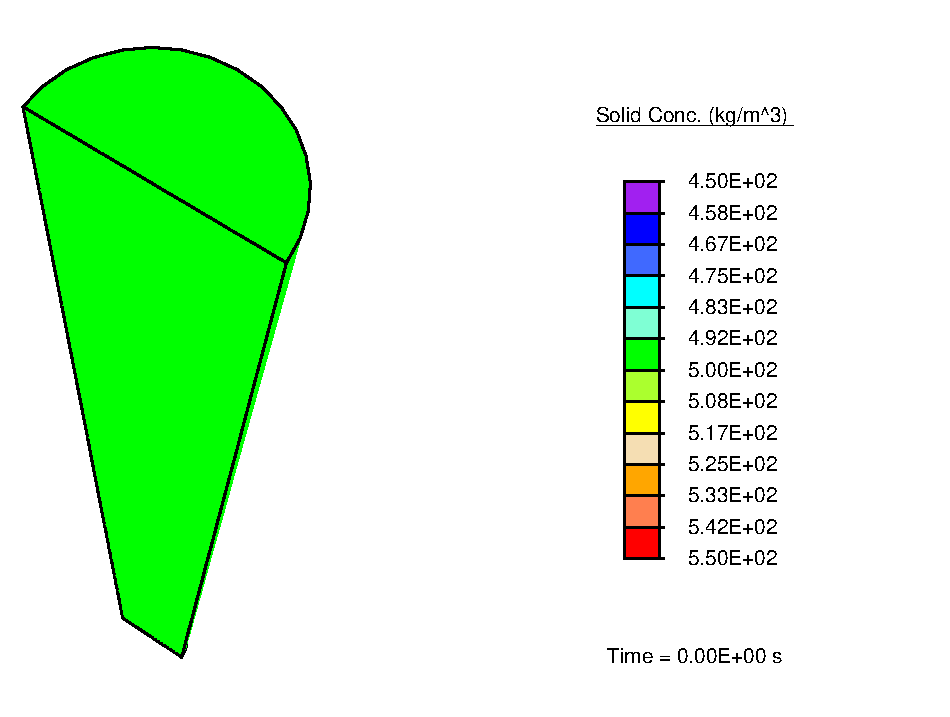
\includegraphics[width=10.00cm]{images/examples/lagrangian/swelling/before-growth}}
     \caption{The collagen initial concentration (kg.m$^{-3}$).}
     \label{before_growth}
\end{figure}

\begin{figure}[ht]
  \centering
     {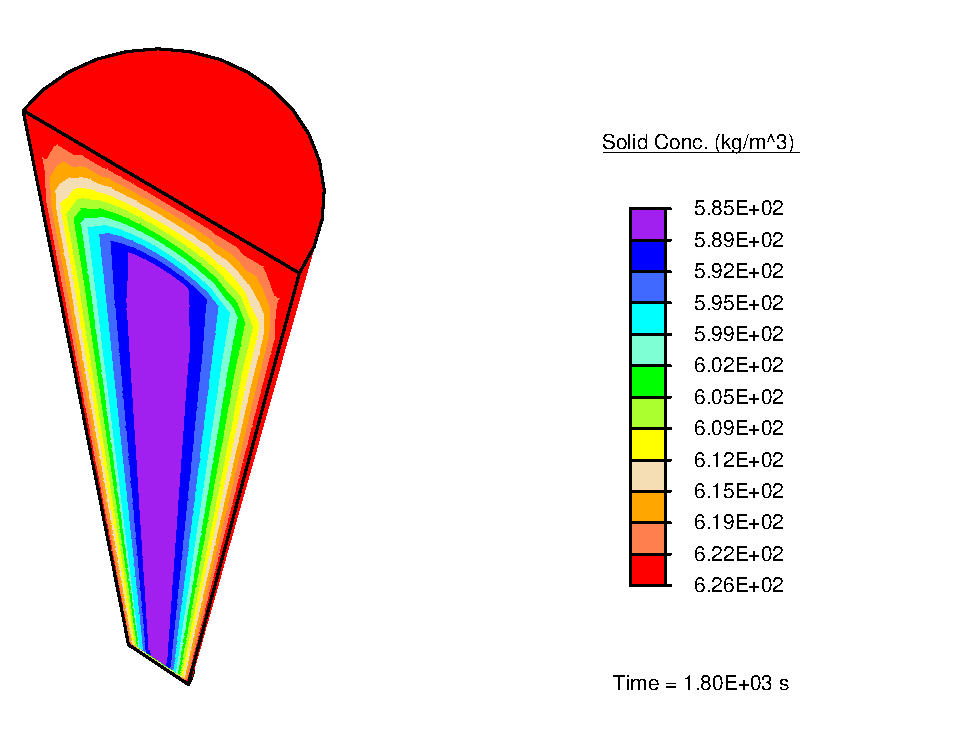
\includegraphics[width=10.00cm]{images/examples/lagrangian/swelling/after-growth}}
     \caption{The collagen concentration (kg.m$^{-3}$) after 1800~s.}
     \label{after_growth}
\end{figure}

\begin{figure}[ht]
  \centering
     {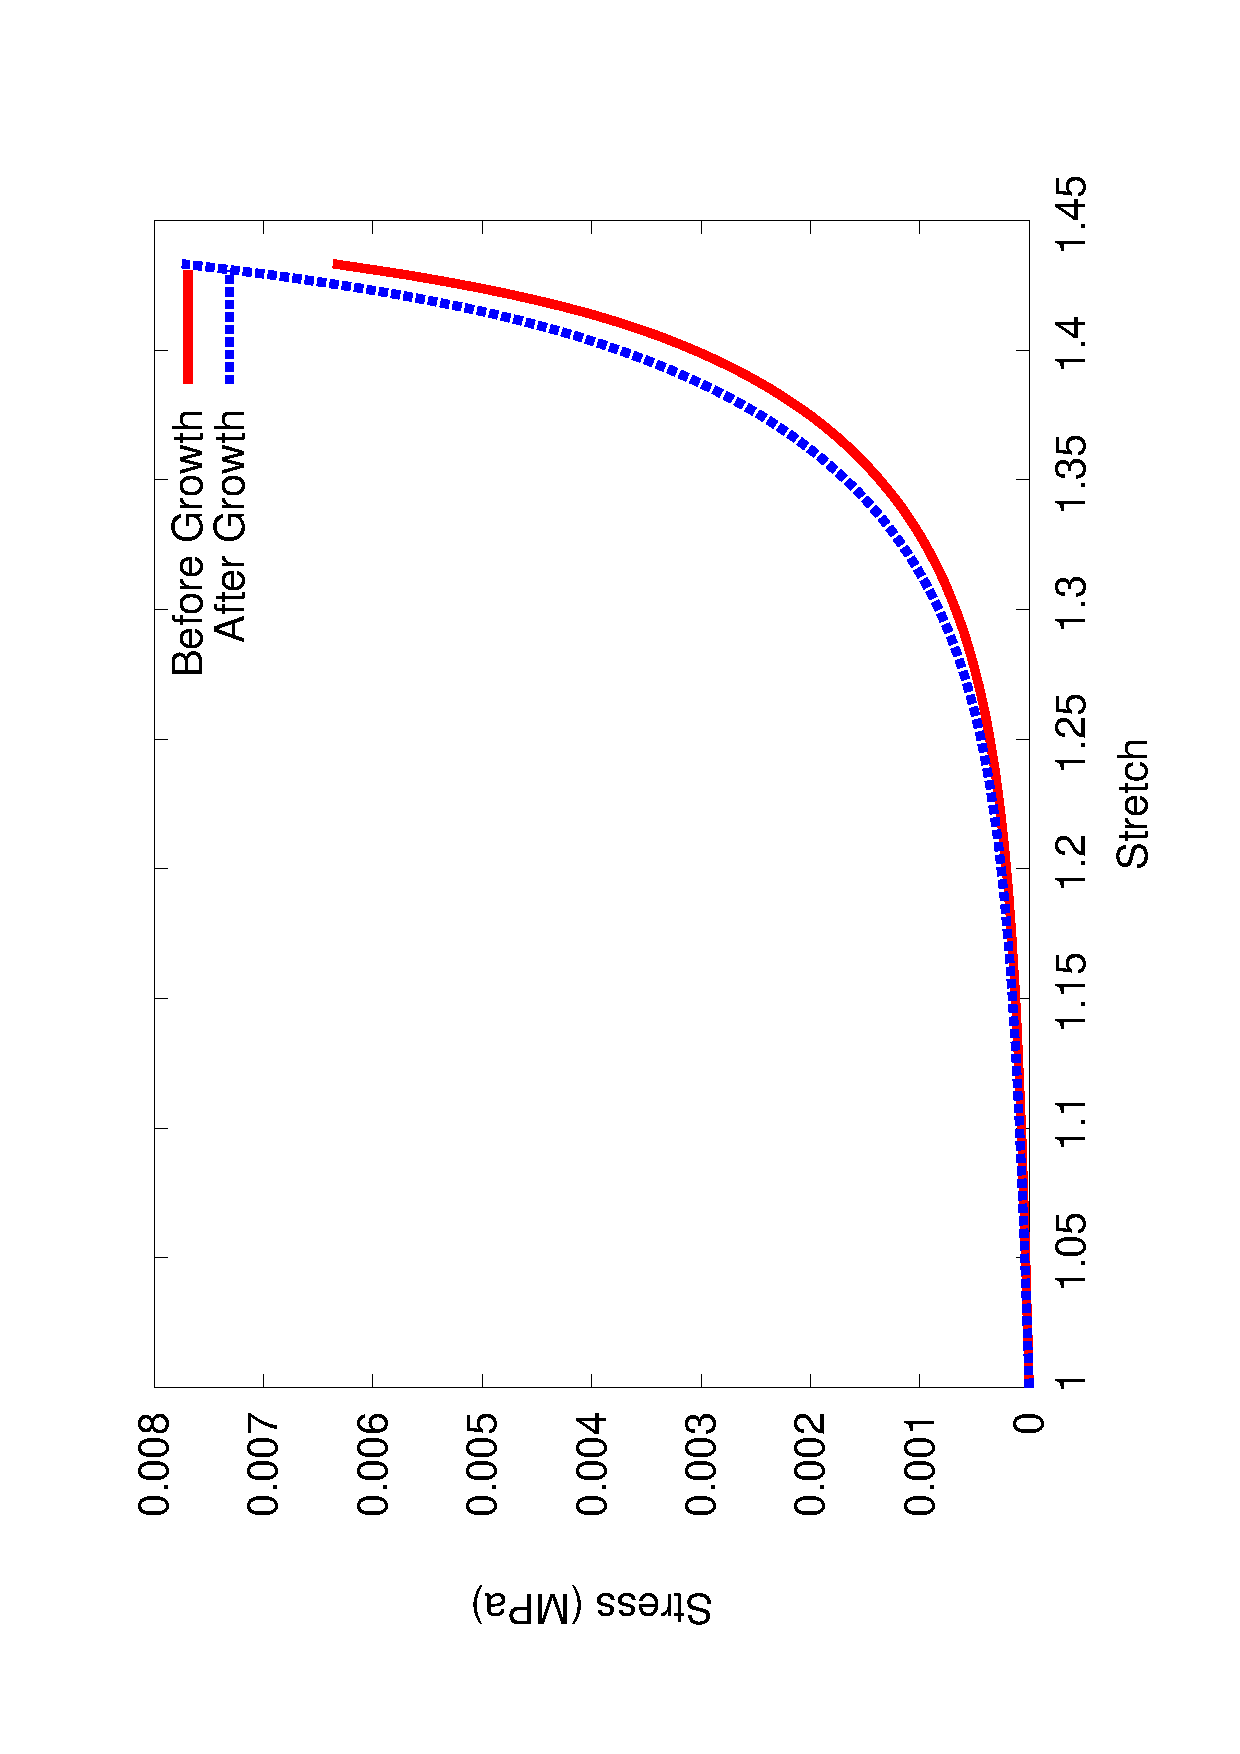
\includegraphics[angle=270,width=10.00cm]{images/examples/lagrangian/swelling/stress-stretch}}
     \caption{The stress (Pa) vs stretch curves before and after
       growth.}
     \label{stress_strain}
\end{figure}

\begin{figure}[ht]
  \centering
     {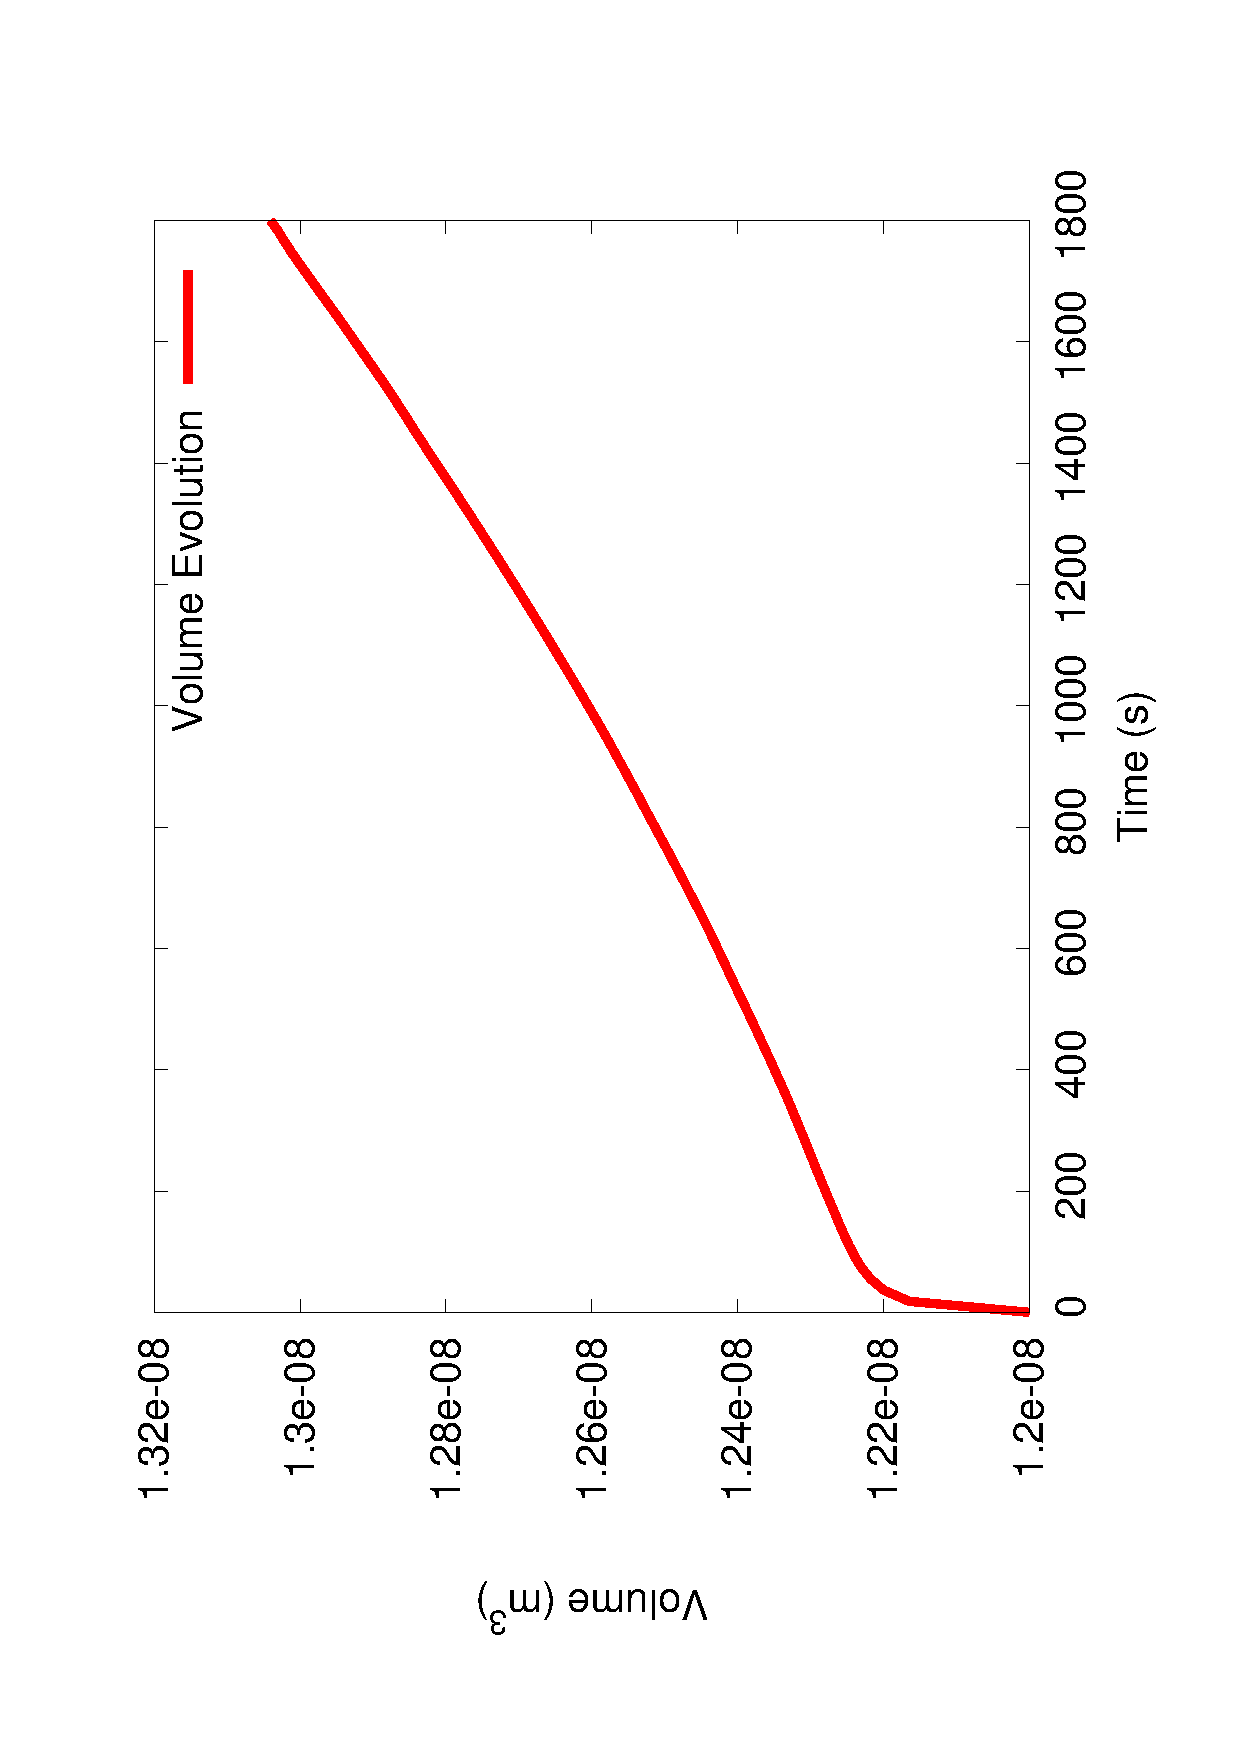
\includegraphics[angle=270,width=10.00cm]{images/examples/lagrangian/swelling/volume-evolution-3}}
     \caption{The volume of the tendon (m$^3$) evolving with
     time. Note the fluid transported-dominated regime until 25 s,
     followed by the longer reaction-dominated growth stage.}
     \label{volume_evolution}
\end{figure}

Motivated mainly by the recognition that the lower bound model for
solid-fluid mechanical coupling ensures convergence to a self-consistent
solution in just a few passes of the staggered solution scheme, we
adopt this version of the coupling for our final problem. On this
  note we point out that solution of the individual balances of linear
  momentum equation for the solid collagenous and fluid phases with
  the momentum transfer terms [$\bq^\mathrm{c}, \bq^\mathrm{f}$ in
  (\ref{linearmombalance})] is a
  statement of momentum balance between them. There is reason to
  suppose, therefore, that equating the solid collagen and fluid
  stress, or some component of these tensors as done in the lower
  bound model, is a reasonable approximation to explicitly solving the
  balance of linear momentum for each phase, including the momentum
  transfers. In contrast, equating the 
  deformation gradient of the solid collagen with deformation of the
  pore spaces subjects the fluid to a stress state also determined by
  this deformation gradient in the upper bound model. This
  approximation does not correspond to an underlying physical
  principle comparable to the satisfaction of individual
  balances of linear momentum for solid collagen and fluid, with
  momentum transfers. It is therefore somewhat less motivated and more
  questionable. Clearly, a rigorous analysis or numerical
  comparisons of all three models:
  upper bound, lower bound and direct solution of individual
  solid-fluid momentum balances, must be carried out to conclusively
  demonstrate this. It is a possible topic for a future paper.

In this example we will demonstrate the mechanical
effects of growth due to collagen production. In the interest of
focusing on this issue we assume that fibroblasts are
available, and that the fluid
phase bears the necessary nutrients for
collagen production dissolved at a suitable, constant
concentration. Collagen production is assumed to be governed by a
first-order rate 
law. Newly-produced collagen has proteoglycan molecules bound to it,
and they in turn bind water. We model this effect by associating a
loss of nutrient-bearing 
free fluid with collagen production. A fluid sink $\Pi^\mathrm{f}$ is
introduced following first order kinetics,

\begin{equation}
\Pi^\mathrm{f} = -k^\mathrm{f}(\rho_0^\mathrm{f}
- \rho_{0_\mathrm{ini}}^\mathrm{f}),
\end{equation}

\noindent as in \citet{growthpaper}. Here $k^\mathrm{f}$ is the
reaction rate, taken to be 0.07 $\mathrm{s}^{-1}$, and
$\rho_{0_\mathrm{ini}}^\mathrm{f}$ is the initial 
concentration of fluid. The collagen
source is mathemaically equivalent to the fluid sink: $\Pi^\mathrm{c} =
-\Pi^\mathrm{f}$. When $\rho_{0}^\mathrm{f} >
\rho_{0_\mathrm{ini}}^\mathrm{f}$, collagen is produced.

The boundary conditions in this example correspond to immersion of the
tendon in a nutrient-rich bath. The initial collagen concentration is
500~kg.m$^{-3}$ and the fluid concentration is 400~kg.m$^{-3}$ at
every point in the tendon. When this tendon is exposed to a bath
where the fluid concentration is 410~kg.m$^{-3}$,
i.e. $\rho^\mathrm{f}(\bx,t)=410~\mathrm{kg.m}^{-3} \forall \bx \in
\partial\Omega_t$, nutrient-rich fluid is transported into the tissue,
due to the pressure difference, induced by the concentration
difference, between the fluid in the tendon and in 
the bath (fluid stress gradient-driven flux). Thereby, the nutrient
concentration is elevated, leading to collagen production, fluid
consumption and, eventually, growth due to additional collagen. 

Figure~\ref{before_growth} shows the initial collagen concentration in
the tendon. After it has been immersed in the nutrient-rich bath for
1800~s, the tendon shows growth and the collagen concentration is
higher as seen in Figure~\ref{after_growth}. On performing a
uniaxial tension test on the tendon before and after growth, it is
observed (Figure~\ref{stress_strain}) that the grown tissue is stiffer
and stronger due to its higher collagen concentration. Also note that
there is a rapid, fluid transport-dominated swelling 
of the tendon  between 0 and 25 s 
following immersion in the fluid bath
(Figure~\ref{volume_evolution}). This causes a small volume change of 
$\approx 1.6$\%. In this transport-dominated regime the contribution
to tendon growth from collagen production is small. However, the
fluid-induced swelling saturates, and between
25 and 1800 s the reaction producing collagen dominates the growth
process, producing a further $\approx 6.8$\% volume change. Noting that the
range of collagen concentration in Figure~\ref{after_growth} is
$585-626\; \mbox{kg.m}^{-3}$, and that (\ref{isotropicgrowth}) gives $\bF^{\mathrm{g}^\mathrm{c}} = \left(
  \frac{\rho_0^\mathrm{c}}{\rho_{0_{\mathrm{ini}}}^\mathrm{c}}
  \right)^  {\frac{1}{3}} {\bf 1}$, this portion of the volume change
  is quite clearly due to collagen production. The total volume change
  of $8.4$\% corresponds to changes in each linear dimension of the
  tendon by only $\approx 2.7$\%, and is not discernible upon comparing
  Figures~\ref{before_growth} and \ref{after_growth}. It is, however,
  manifest in Figure~\ref{volume_evolution}.

\section{A multiphasic problem based on enzyme-kinetics}
\label{enzyme-kinetics}

\begin{table}
\centering
\begin{tabular}{lll}
\hline
\multicolumn{1}{c}{Parameter (Symbol)} & Value & Units\\
\hline
Chain density ($N$) & $7\times 10^{21}$ & $\mathrm{m}^{-3}$\\
Temperature ($\theta$)  & $310.6$ & K\\
Persistence length ($A$) & $2.10$ & --\\
Fully-stretched length ($L$) & $2.125$ & --\\
Unit cell axes ($a,\;b,\;c$) & $1.95,\;1.95,\;2.43$ & --\\
Bulk compressibility factors ($\gamma,\;\beta$) & $1000,\; 4.5$ & --\\
Fluid bulk modulus ($\kappa^f$) & $1$ & GPa\\
Fluid mobility tensor ($D^\mathrm{f}_{ij} = D^\mathrm{f}\delta_{ij}$) & $1\times 10^{-14}$
&s\\
%Fluid mol. wt. ($\sM^\mathrm{f}$)& $2.991\times 10^{-26}$ & $\mathrm{kg}$\\ 
Fibroblast concentration ($\rho_{\mathrm{cell}}$) & 0.2 &
kg.m$^{-3}$\\
Max. reaction rate ($k_{\mathrm{max}} = 5$) & 5 & s$^{-1}$\\
Max. solute concentration ($\rho^{\mathrm{s}}_m$) & 0.2 &
kg.m$^{-3}$\\
Solute diffusivity ($\bD^\mathrm{s}$) & $1\times 10^{-9}$ &  m$^{-2}$s\\
\hline
\end{tabular}
\caption{Material parameters used in the analysis.}
\label{parameters}
\end{table}

This first example can be viewed as a model for localised, bolus
delivery of regulatory chemicals to the tendon while accounting for
mechanical (stress) effects. A single solute species\footnote{Here, we
  envision the solute to be a protein playing 
  an essential role in growth by catalysing underlying biochemical
  reactions. An important example of this is a family of proteins,
  TGF$\beta$, which is a multi-functional peptide that controls numerous
  functions of many cell types \citep{Alberts:02}.} is considered,
denoted by s, and 
a uniform distribution of fibroblasts that are characterised by their
cell concentration, $\rho_{\mathrm{cell}}$. Both, Fickean diffusion of
the solute, and stress gradient driven fluid flow are incorporated in this
illustration. We use 
Michaelis-Menten enzyme kinetics [Equation~(\ref{enzymekineticseq})]
to determine the rates of solute consumption and collagen production
as a function of solute concentration. This non-linear relationship for
our choice of parameters is visualised in
Figure~\ref{eg3menten}. Here, the fluid phase does not  take part in
reactions, and hence $\Pi^\mathrm{f}=0$. 

\begin{figure}
\centering
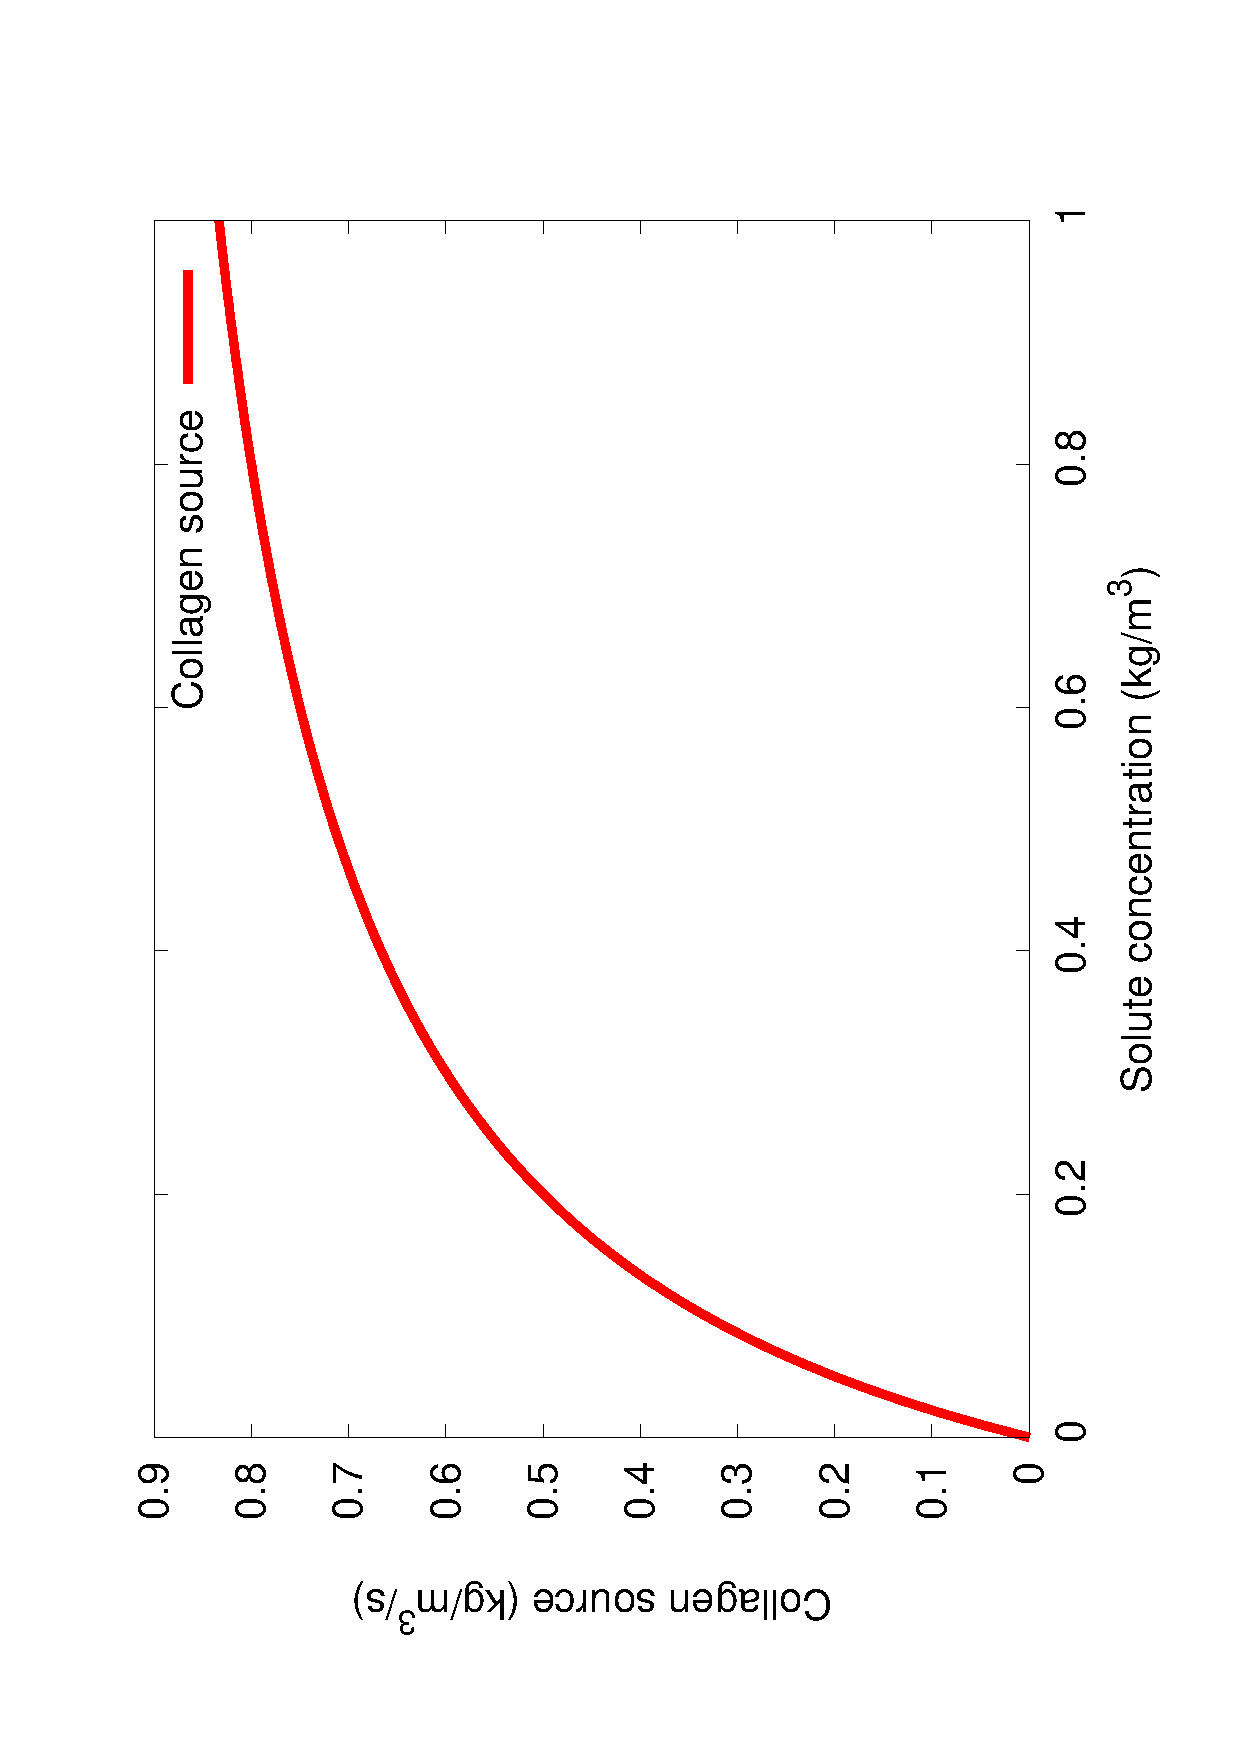
\includegraphics[angle=270,width=10.00cm]{images/elucidation/enzyme-kinetics}
\caption{Variation of the collagen source term (kg.m$^{-3}$.s$^{-1}$)
  with solute concentration (kg.m$^{-3}$).}
\label{eg3menten}
\end{figure}

The tendon immersed in the bath is subjected to a constrictive
radial load, such
as would be imposed upon  manipulating it with a set of tweezers, as depicted in
Figure~\ref{constrictload}. The
maximum strain in the radial 
direction---experienced half-way through the height of the tendon---is
10\%. The applied strain in the radial direction decreases linearly
with distance from the central plane, and vanishes at the top and
bottom surfaces of the tendon. 


\begin{figure}[ht]
  \centering
  \psfrag{M}{\small $\bN\cdot\bM^f$}
  \psfrag{P}{\small ${\tiny\quad }~\bu$}
         {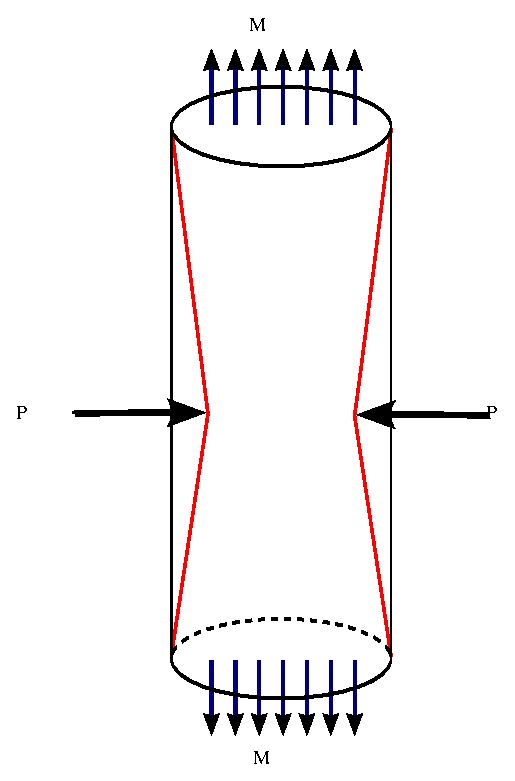
\includegraphics[width=5.0cm]{images/examples/lagrangian/constriction/cylinder-in-bath}}
	 \caption{Constrictive load applied to tendon immersed in a
	 bath.} 
	 \label{constrictload}
\end{figure}

The 
initial collagen concentration and the initial fluid concentration are
both 500~kg.m$^{-3}$ at every point in the tendon, and the fluid
concentration in the bath is 500~kg.m$^{-3}$. In
addition, a solute-rich bulb of radius 0.15~mm is introduced with
its centre on the axis of the tendon and situated 3~mm below the upper
circular face of the tendon. The initial solute concentration is
0.05~kg.m$^{-3}$ at all other points in the tendon, and increases
linearly with decreasing radius in this bulb to 1~kg.m$^{-3}$ at its
centre (see Figure~\ref{eg3ini}). The
parameters used are listed in Table~\ref{parameters}, and are relevant
to tendons.

\begin{figure}
\centering
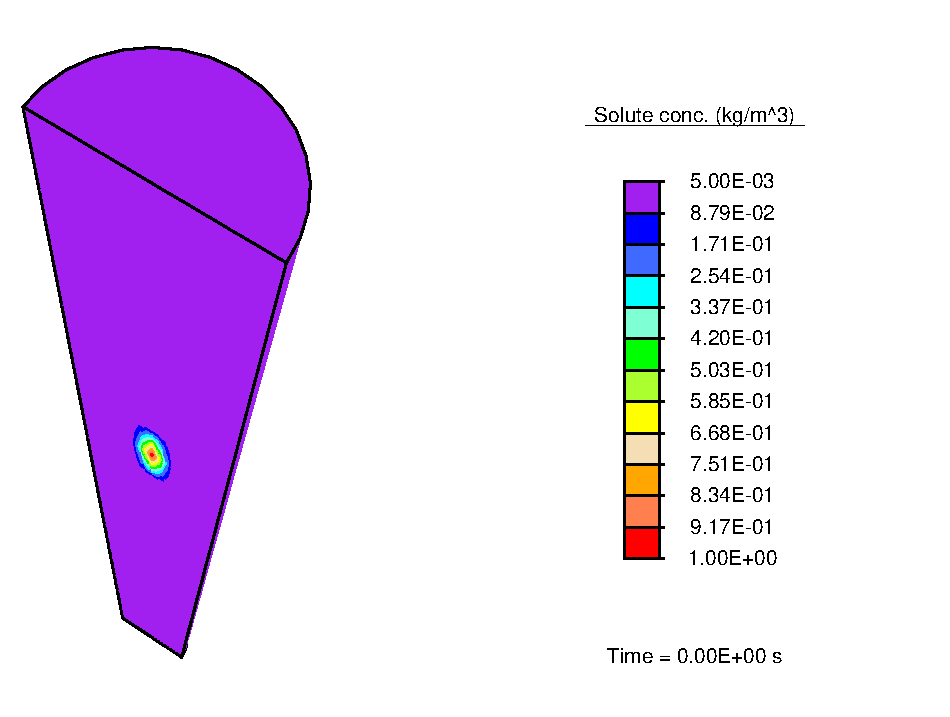
\includegraphics[width=10.00cm]{images/examples/lagrangian/medication/initial-solute-concentration}
\caption{The solute concentration (kg.m$^{-3}$) initially.}
\label{eg3ini}
\end{figure}

The aim of this example is to compare the influences upon solute
transport from two mechanisms: Fluid stress gradient-driven transport,
arising from the applied constrictive load, and solute concentration
gradient-driven transport. These mechanisms have both been implicated
in nutrient supply to cells in soft tissue. The results of this
numerical example demonstrate that because the magnitude of the fluid mobility
for stress gradient driven transport is orders of magnitude
smaller than the diffusion coefficient for the solute through the
fluid, there is relatively only a small stress gradient driven flux,
and the transport of the solute is diffusion dominated. As a result,
the solute diffuses locally, but displays no
observable advection along the fluid. As the diffusion-driven solute
concentration in a region increases, the enzyme-kinetics model
results in a small source term for collagen production, and we observe nominal
growth. Figure~\ref{eg3conc} shows the collagen concentration at an
early time, $t=5\times10^{-2}$~s.

\begin{figure}
\centering
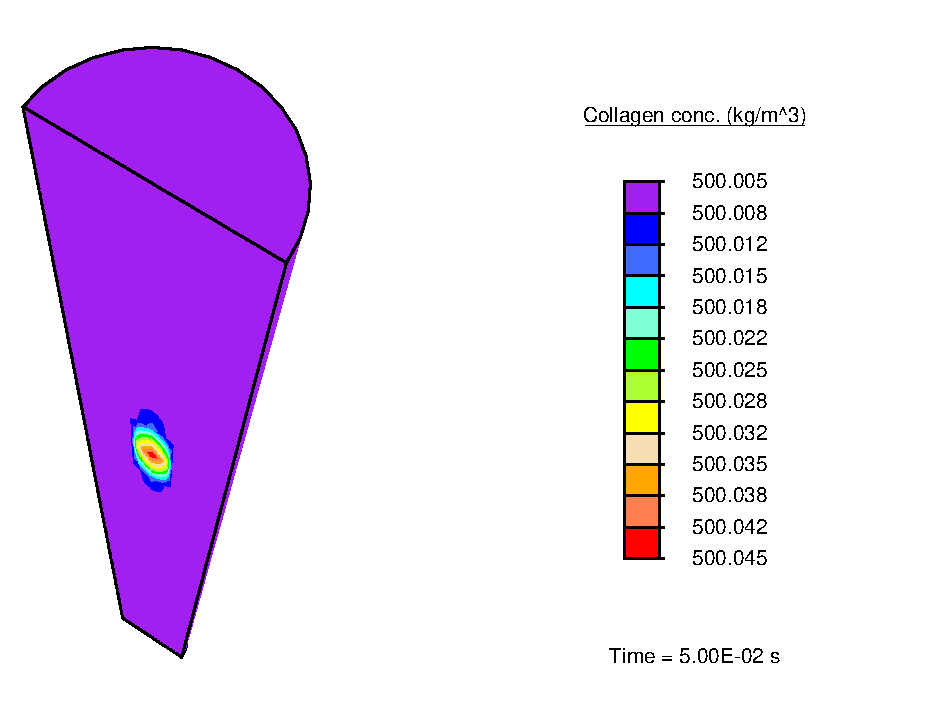
\includegraphics[width=10.00cm]{images/examples/lagrangian/medication/final-collagen-concentration}
\caption{The collagen concentration (kg.m$^{-3}$) at time
  $t=5\times10^{-2}$~s.}
\label{eg3conc}
\end{figure}

This example incorporates all of the theory discussed in the
paper. However, it is a valuable exercise in
modelling to simplify the boundary value problem, and supress some of
the coupled phenomena in order to gain a better understanding of some
effcts. This is the approach followed in the next two numerical
examples. The detailed transport and mechanics induced by the
constrictive radial load are discussed first in Section~\ref{pinching}. 

\section{Wound healing}
\label{wound-healing}

%

% Local Variables:
% TeX-master: "thesis"
% mode: latex
% mode: flyspell
% End:
